\documentclass[a4paper,12pt]{article}
\usepackage[utf8]{inputenc}
\setlength{\marginparwidth}{2cm}
\usepackage{todonotes}
\usepackage[russian]{babel}
\usepackage{graphicx}
\usepackage{amsmath, amssymb}
\usepackage{hyperref}
\usepackage{float}
\usepackage{listings}
\usepackage{caption}
\usepackage{geometry}
\usepackage{xcolor}
\geometry{left=2cm,right=2cm,top=2cm,bottom=2cm}
\hypersetup{pdfborder=0 0 0}
\headsep=8mm
\footskip=20mm
\hypersetup{pdfstartview=FitH, linkcolor=linkcolor, urlcolor=urlcolor, colorlinks=true}

\definecolor{strings}{rgb}{0,0.6,0}
\definecolor{comments}{rgb}{0,0.3,0}
\definecolor{numbers}{rgb}{0.5,0.5,0.5}
\definecolor{keywords}{rgb}{0.09,0.61,0.95}
\definecolor{background}{rgb}{0.97,0.97,0.97}

\lstdefinestyle{codestyle}{
    backgroundcolor=\color{background},
    commentstyle=\color{comments},
    keywordstyle=\color{keywords},
    stringstyle=\color{strings},
    numberstyle=\tiny\color{numbers},
    basicstyle=\ttfamily\scriptsize,
    breakatwhitespace=false,
    breaklines=true,
    captionpos=b,
    inputencoding=utf8,
    keepspaces=false,
    numbers=left,
    numbersep=5pt,
    showspaces=false,
    showstringspaces=false,
    showtabs=false,
    tabsize=2,
    extendedchars=true
}

\lstset{style=codestyle}

\begin{document}    

% Титульный лист
\begin{titlepage}
    \centering
    {\large Федеральное государственное автономное образовательное учреждение\par}
    {\large высшего образования\par}
    {\bfseries САНКТ-ПЕТЕРБУРГСКИЙ НАЦИОНАЛЬНЫЙ ИССЛЕДОВАТЕЛЬСКИЙ УНИВЕРСИТЕТ ИТМО\par}
    {\bfseries Факультет систем управления и робототехники\par}
    \vfill
    {\Large \bfseries Лабораторная работа №2\par}
    {\Large \bfseries Метод Ньютона \par}
    \vfill
    
    \begin{flushright}
        Студенты: Бахтаиров Р.А.,\\ Сайфуллин Д.Р. \\
        Группа:  R3243\\
        Преподаватель: Попов А.М.
    \end{flushright}
    \vfill
    Санкт-Петербург\\ 
    2025 г.
\end{titlepage}

\section{Введение}
Целью данной лабораторной работы является разработка и исследование численных методов оптимизации, в частности метода Ньютона, для нахождения минимума функций.
\textit{Примечание: весь код для выполнения работы находится в файле \texttt{main.ipynb}.}

\section{Численное нахождение градиента и гессиана}
Для выполнения задания необходимо реализовать численное нахождение градиента и гессиана функции $f(x)$ в точке $x$. Проверим реализованные методы и оценим зависимость точности градиента и гессиана от выбора шага $h$ на следующих тестовых функциях:
\begin{enumerate}
    \item[(a)] $f_1(x) = \sin(x) + \cos(y),\\ [0.5em]
        \text{Градиент: } \nabla f_1(x,y) = \left( \cos(x), -\sin(y) \right), \\
        \text{Гессиан: } \nabla^2 f_1(x,y) = \begin{pmatrix}
        -\sin(x) & 0 \\
        0 & -\cos(y)
        \end{pmatrix}$

    \item[(b)] $f_2(x) = x_0^3 + x_1^3 + x_2^3,\\ [0.5em]
        \text{Градиент: } \nabla f_2(x) = \left( 3x_0^2,\, 3x_1^2,\, 3x_2^2 \right) \\
        \text{Гессиан: } \nabla^2 f_2(x) = \begin{pmatrix}
            6x_0 & 0 & 0 \\
            0 & 6x_1 & 0 \\
            0 & 0 & 6x_2
            \end{pmatrix}$ \\
        Особенностью полинома третьей степени является то, что его разложение в ряд Тейлора совпадает с исходной функцией, что приводит к теоретической точности схем конечных разностей для любого шага \( h \).
    \item[(c)] $f_3(x) = \exp(x_0) + \ln(1+x_1) + \arctan(x_2) + x_2^2, \\ [0.5em]
        \text{Градиент: } \nabla f_3(x) = \left( \exp(x_0),\, \frac{1}{1+x_1},\, \frac{1}{1+x_2^2}+2x_2 \right),\\
        \text{Гессиан: } \nabla^2 f_3(x) = \begin{pmatrix}
            \exp(x_0) & 0 & 0 \\
            0 & -\frac{1}{(1+x_1)^2} & 0 \\
            0 & 0 & -\frac{2x_2}{(1+x_2^2)^2}+2
            \end{pmatrix}$
\end{enumerate} 

\subsection{Первая производная (градиент)}
Для дифференцируемой функции \( f(x) \) одной переменной центральная разностная схема даёт приближение первой производной:
\[
f'(x) \approx \frac{f(x+h) - f(x-h)}{2h},
\]
где \( h \) --- малый шаг. Для функции нескольких переменных вектор градиента \( \nabla f(x) \) можно получить, вычисляя частные производные по каждой координате:
\[
\frac{\partial f}{\partial x_i}(x) \approx \frac{f(x+he_i) - f(x-he_i)}{2h},
\]
где \( e_i \) --- единичный вектор по \( i \)-й координате.

\subsection{Вторая производная (гессиан)}  
Для функции одной переменной вторая производная аппроксимируется по формуле:
\[
f''(x) \approx \frac{f(x+h)-2f(x)+f(x-h)}{h^2}.
\]
Для функции нескольких переменных второй порядок частных производных оценивается по формуле:
\[
\frac{\partial^2 f}{\partial x_i \partial x_j}(x) \approx \frac{f(x+he_i+he_j)-f(x+he_i-he_j)-f(x-he_i+he_j)+f(x-he_i-he_j)}{4h^2}.
\]
Из этих частных производных составляется матрица Гессе \( \nabla^2 f(x) \). Важно отметить, что для дважды непрерывно дифференцируемых функций матрица Гессе является симметричной.


\subsection{Анализ}
В задании проводится оценка зависимости точности численного вычисления градиента и гессиана от выбора шага \( h \). Для каждой из выбранных функций эксперимент производится следующим образом:
\begin{itemize}
    \item Задаётся диапазон шагов \( h \) в виде вещественных чисел, после чего для построения графиков ось абсцисс переводится в логарифмическую шкалу.
    \item Для каждой функции вычисляются численный градиент и гессиан в заданной точке, и вычисляется норма разности между численным результатом и аналитически найденными значениями.
    \item Результаты визуализируются в виде двух графиков: один для ошибки градиента и второй для ошибки гессиана, что позволяет оценить оптимальный диапазон выбора шага \( h \) и влияние машинного округления на точность вычислений.
\end{itemize}
\begin{figure}[H]
    \centering 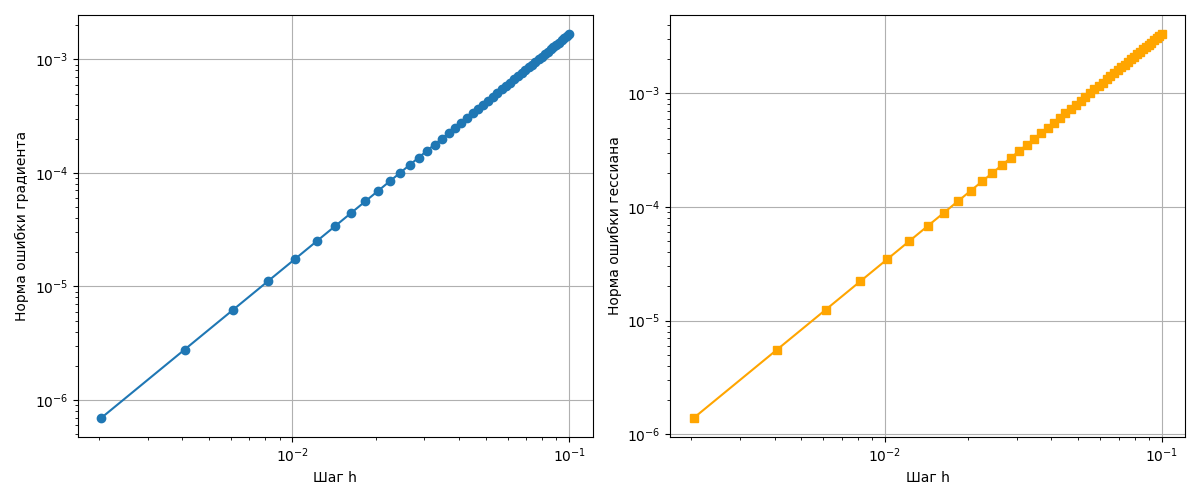
\includegraphics[width=\textwidth]{images/1_f1.png}
    \caption{Ошибка градиента и гессиана для $f_1$}
\end{figure}
\noindent На графиках для функции \( f_1 \) наблюдаются следующие тенденции:
\begin{itemize}
    \item Градиент: При небольших значениях \(h\) ошибка невысока. По мере увеличения \(h\) ошибка постепенно растёт, так как шаг становится слишком большим для точного вычисления разностей.
    \item Гессиан: Ситуация похожая на градиент. В представленной области ошибок наблюдается плавный рост при увеличении \(h\).
\end{itemize}
Для \(f_1\) более мелкий шаг \(h\) даёт более точные результаты, а при больших \(h\) ошибка возрастает.

\begin{figure}[H]
    \centering 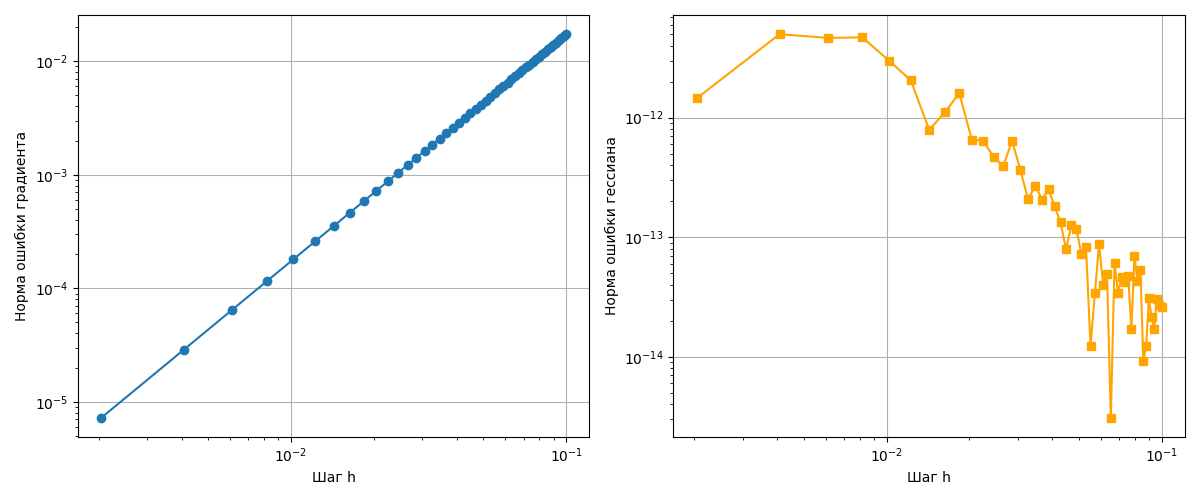
\includegraphics[width=\textwidth]{images/1_f2.png}
    \caption{Ошибка градиента и гессиана для $f_2$}
\end{figure}
\noindent На графиках для функции \( f_2 \) наблюдаются следующее:
\begin{itemize}
    \item Градиент: Ошибка при вычислении градиента ведет себя схоже с \(f_1\). При малых значениях \(h\) ошибка невысока, но при увеличении шага ошибка растёт.
    \item Гессиан: Ошибка гессиана практически равна нулю, так как для кубического полинома аналитически вторая производная вычисляется очень точно.
\end{itemize}
Для \(f_2\) численные методы дают практически идеальные результаты, особенно для гессиана.

\begin{figure}[H]
    \centering 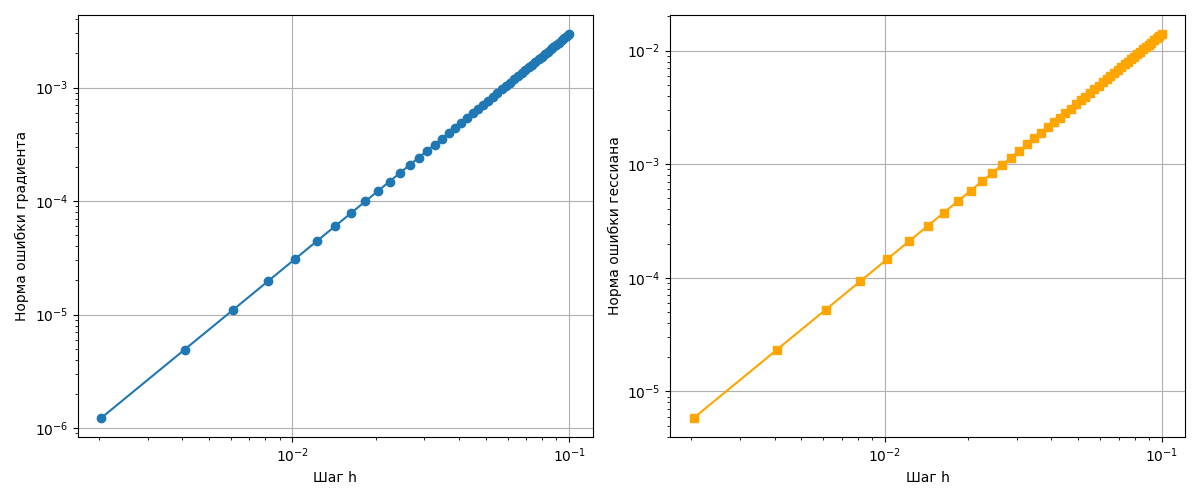
\includegraphics[width=\textwidth]{images/1_f3.png}
    \caption{Ошибка градиента и гессиана для $f_3$}
\end{figure}
\noindent На графиках для функции \( f_3 \) наблюдаем:
\begin{itemize}
    \item Градиент График показывает, что ошибка растёт с увеличением \(h\). При небольшом \(h\) ошибка минимальна, а при больших значениях \(h\) приближение становится менее точным.
    \item Гессиан: Аналогично, ошибка гессиана увеличивается при увеличении \(h\). Здесь функция сложнее, поэтому точность численного метода чувствительна к выбору шага.
\end{itemize}
Для \(f_3\) оптимальное значение \(h\) очень важно, так как слишком большой шаг резко увеличивает ошибку.

\begin{figure}[H]
    \centering 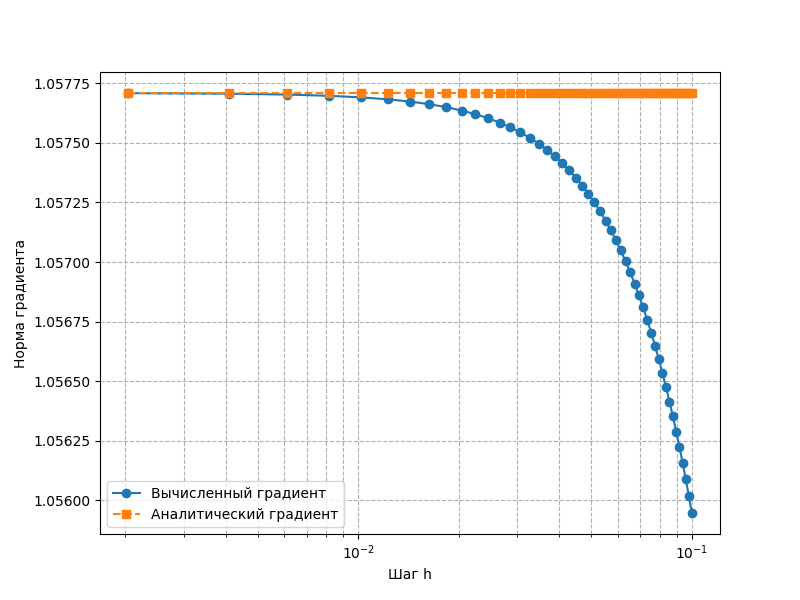
\includegraphics[width=\textwidth]{images/comp.png}
    \caption{Зависимость нормы градиента от шага \(h\)}
\end{figure}
\noindent На рисунке выше мы показали зависимость нормы вычисленного градиента от шага \(h\) в сравнении с постоянным уровнем аналитической нормы градиента. Видно, что при относительно малых значениях \(h\) (в левой части графика) вычисленный градиент практически совпадает с аналитическим. Однако по мере увеличения \(h\) значение нормы численно вычисленного градиента постепенно убывает и всё сильнее отдаляется от истинного уровня.
\begin{itemize}
    \item При \( h < 10^{-2}\) значения вычисленного и аналитического градиентов практически совпадают, указывая на то, что центральная разностная схема даёт точное приближение.
    \item При дальнейшем увеличении \(h\) становится заметным занижение нормы вычисленного градиента, так как разностная формула перестаёт отражать истинное локальное поведение функции. В этом режиме шаг \(h\) слишком велик, и аппроксимация производной становится неточной.
\end{itemize}
 

Теперь необходимо предложить функцию \(f: \mathbb{R}^n \to \mathbb{R}\), вычисление которой и её производных (градиента и гессиана) будет иметь вычислительную сложность, растущую линейно с увеличением размерности \(n\).

Рассмотрим функцию
\[
f(x) = \sum_{i=1}^{n} x_i^2,
\]
где \(x = (x_1, x_2, \dots, x_n) \in \mathbb{R}^n\). Такая функция обладает следующими свойствами:
\begin{itemize}
    \item Вычисление функции: Для вычисления \(f(x)\) необходимо просуммировать \(n\) квадратов, что требует \(O(n)\) операций.
    \item Градиент: Аналитически градиент функции равен
    \[
    \nabla f(x) = (2x_1, 2x_2, \dots, 2x_n).
    \]
    Вычисление этого вектора также требует \(O(n)\) операций.
    \item Гессиан: Аналитический гессиан функции представляет собой диагональную матрицу:
    \[
    \nabla^2 f(x) = 2I_n,
    \]
    где \(I_n\) --- единичная матрица размерности \(n\).
\end{itemize}

\begin{figure}[H]
    \centering 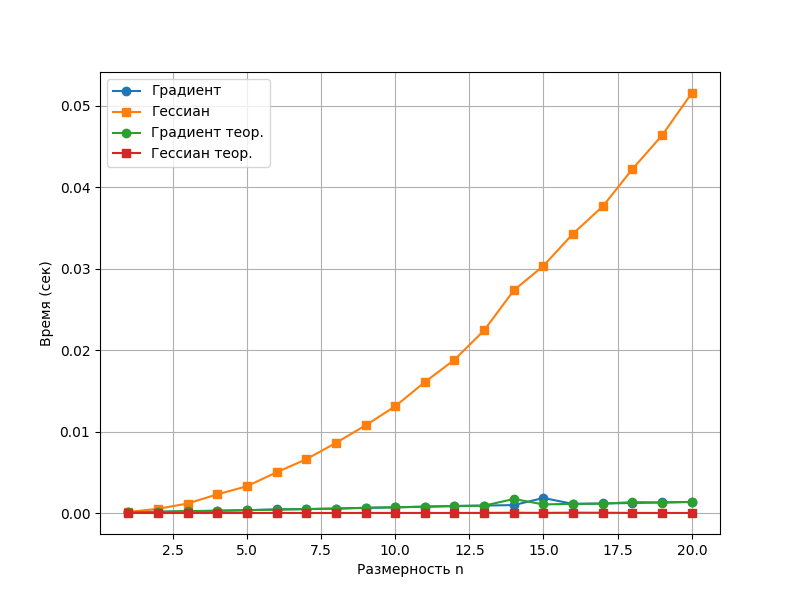
\includegraphics[width=\textwidth]{images/tick.png}
    \caption{Зависимость времени вычислений от размерности $n$}
\end{figure}
На приведённом графике наблюдается следующая зависимость времени вычислений от размерности \(n\):

\begin{itemize}
    \item Время вычисления градиента растёт примерно линейно с увеличением \(n\). Это соответствует теоретической оценке сложности \(O(n)\), так как для вычисления градиента производится проход по всем \(n\) компонентам.
    \item Время вычисления гессиана растёт значительно быстрее, что указывает на квадратичную зависимость \(O(n^2)\).
\end{itemize}

\noindent Мы экспериментально подтвердили, что вычисление градиента имеет линейную сложность \(O(n)\), а вычисление гессиана методом центральных разностей --- квадратичную сложность \(O(n^2)\). При больших размерностях \(n\) затраты на вычисление гессиана существенно возрастают, что следует учитывать при выборе численных методов в задачах оптимизации.

\section{Метод Ньютона}
Метод Ньютона является одним из классических итерационных методов решения задач оптимизации, основанных на использовании информации о второй производной функции. Основная идея метода заключается в том, что на каждом шаге текущая точка обновляется согласно правилу
\[
x_{k+1} = x_k - \alpha \, \left(\nabla^2 f(x_k)\right)^{-1} \nabla f(x_k),
\]
где \(\nabla f(x_k)\) — градиент, \(\nabla^2 f(x_k)\) — гессиан функции \(f\) в точке \(x_k\), а \(\alpha\) — коэффициент шага. Метод Ньютона обладает квадратичной сходимостью вблизи оптимума, что делает его весьма эффективным при условии, что вычисление градиента и гессиана не является слишком затратным.

В данном задании метод Ньютона реализован в двух вариантах:
\begin{itemize}
    \item с фиксированным шагом \(\alpha = 1\);
    \item с адаптивным подбором шага по стратегии Армихо--Вульфа.
\end{itemize}
Для тестирования метода рассматриваются задачи оптимизации для квадратичных функций, а также для функций с более сложной структурой, что позволяет оценить как поведение метода, так и влияние выбора параметров на сходимость алгоритма.

Рассмотрим функцию вида
\[
f(x) = x^T \begin{pmatrix} 3.0 & 1.0 \\[6pt] 1.0 & 2.0 \end{pmatrix} x \;+\; 
\begin{pmatrix}-2.0 \\[2pt] 1.0\end{pmatrix}^T x,
\]
с начальными значениями \(x_0 = (2.5, 7.5)\). 

\begin{figure}[H]
    \centering
    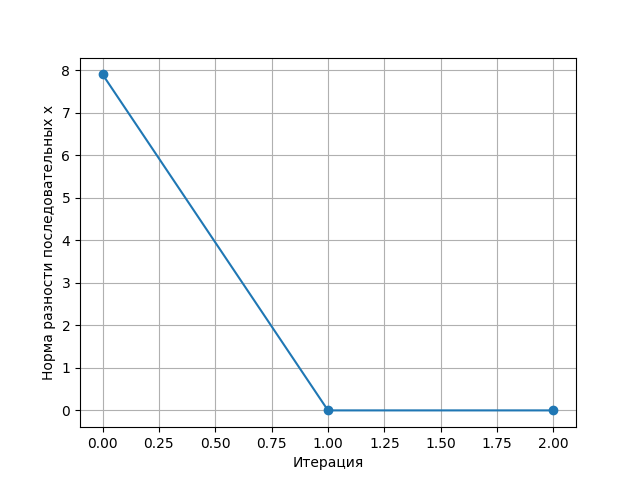
\includegraphics[width=\textwidth]{images/quad_convergence.png}
    \caption{Сходимость метода Ньютона на квадратичной функции: норма \(\|x_{k+1} - x_k\|\) по итерациям.}
\end{figure}
\noindent На графике ниже показана норма разности векторов \(x_k\) на соседних итерациях. Видно, что уже к первой итерации величина скачка падает практически до нуля, а к следующей итерации решение стабилизируется. Это указывает на быструю сходимость метода Ньютона для квадратичных функций: фактически за один шаг мы переходим от далёкой начальной точки \((2.5, 7.5)\) к окрестности оптимума.

\begin{figure}[H]
    \centering
    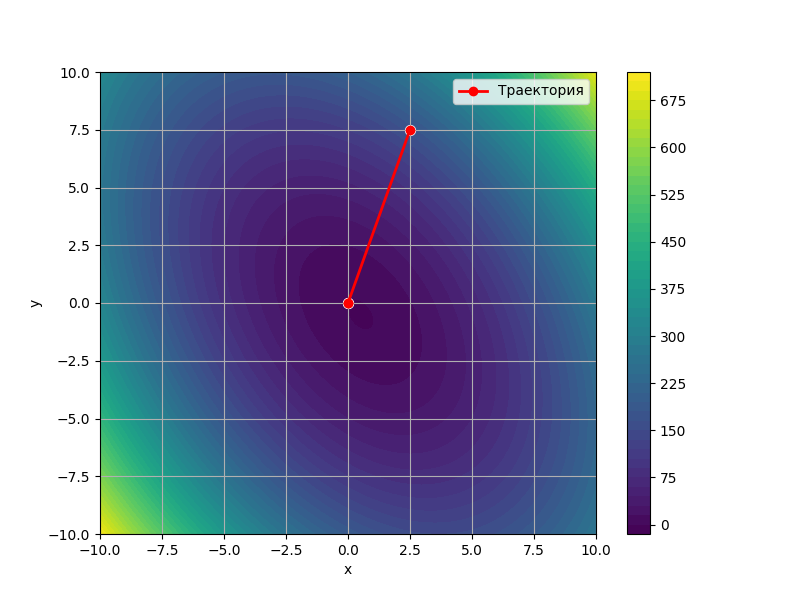
\includegraphics[width=\textwidth]{images/quad_contour.png}
    \caption{Контурный график рассматриваемой квадратичной функции с отмеченной траекторией итераций.}
\end{figure}
\noindent На  представлен контурный график функции с отмеченными точками траектории. Исходная точка \((2.5, 7.5)\) расположена далеко от минимума, но метод Ньютона делает один «крупный» шаг, быстро переходя ближе к оптимуму, а затем одним дополнительным шагом достигает решения с высокой точностью. 

Теперь рассмотрим функцию
\[
f(x,y)=-\frac{1}{1+(x-a)^2+(y-b)^2}
\]
параметры \(a\) и \(b\) выбираются согласно условию. Основная цель --- изучить поведение метода Ньютона при использовании фиксированного шага и при адаптивном подборе шага.

\begin{figure}[H]
    \centering
    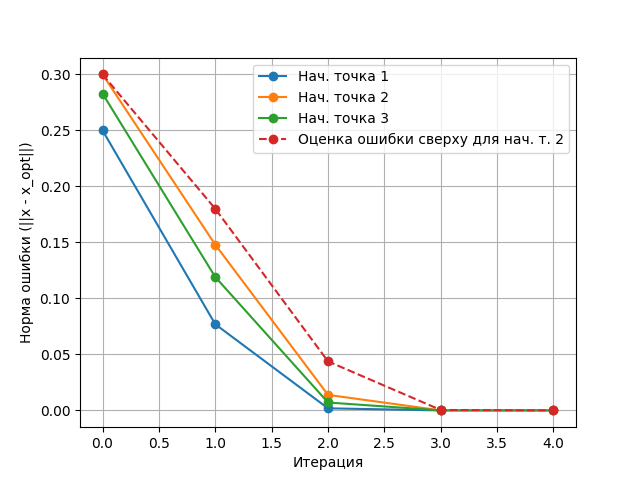
\includegraphics[width=0.8\textwidth]{images/newton_fixed_conv.png}
    \caption{График сходимости метода Ньютона с фиксированным шагом \(\alpha=1\).}
\end{figure}
\noindent На данном графике видно, что при фиксированном шаге \(\alpha=1\) норма разности между последовательными итерациями быстро снижается в начальных шагах, что свидетельствует о резком приближении к оптимуму.

\begin{figure}[H]
    \centering
    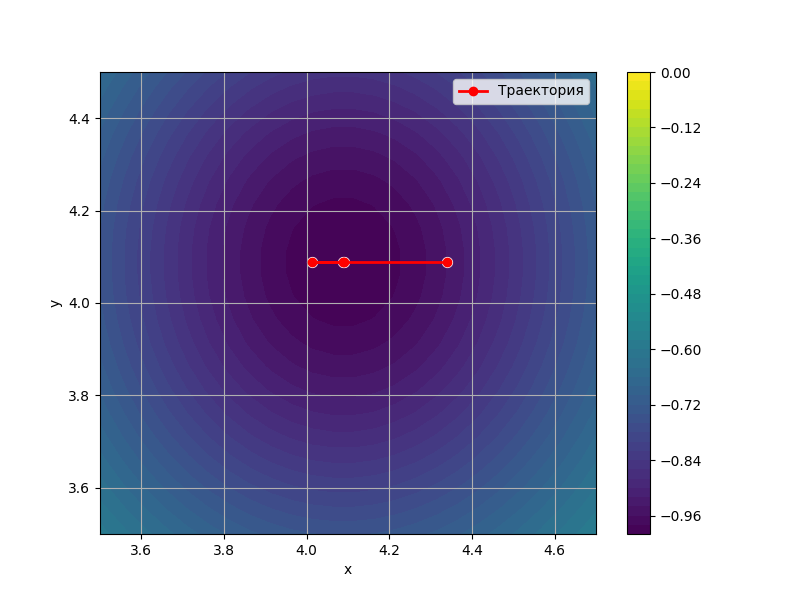
\includegraphics[width=0.8\textwidth]{images/newton_fixed_traj.png}
    \caption{Траектория итераций метода Ньютона с фиксированным шагом \(\alpha=1\) для начальной точки 2.}
\end{figure}
\noindent Контурный график демонстрирует, что при использовании фиксированного шага траектория итераций проходит резким "скачком" от начальной точки к области, где расположен оптимум. Итерационный путь выглядит ломано, что указывает на то, что фиксированный шаг не всегда оптимально соответствует локальной кривизне функции. Несмотря на это, конечная точка итерационного процесса оказывается достаточно близко к оптимальному решению.

\begin{figure}[H]
    \centering
    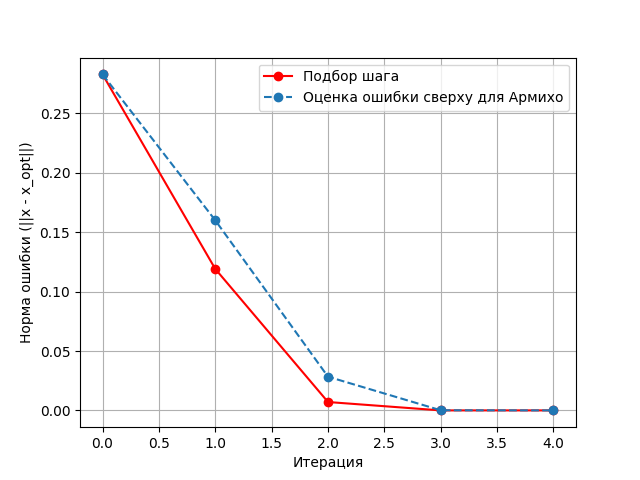
\includegraphics[width=0.8\textwidth]{images/newton_adaptive_conv.png}
    \caption{График сходимости метода Ньютона с адаптивным подбором шага.}
    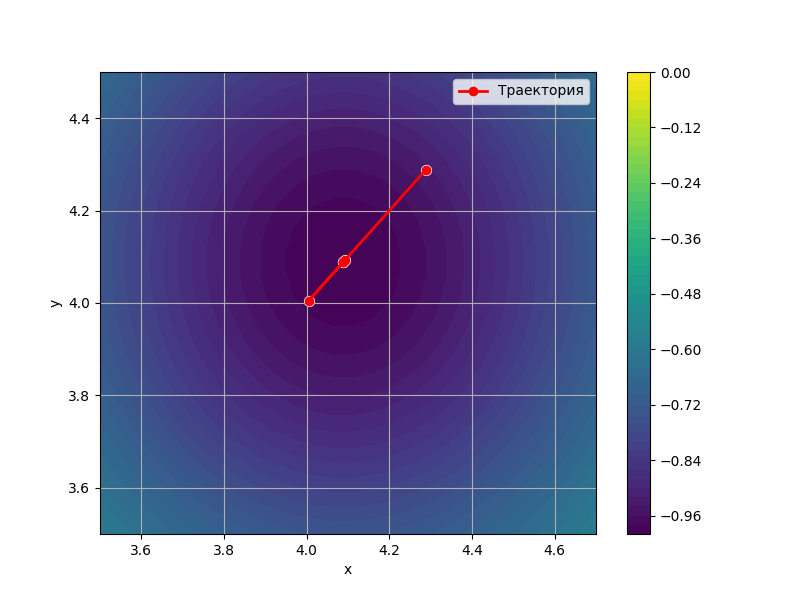
\includegraphics[width=0.8\textwidth]{images/newton_adaptive_traj.png}
    \caption{Траектория итераций метода Ньютона с адаптивным подбором шага.}
\end{figure}
\noindent Графики выше с адаптивным подбором шага показывают более гладкую и непрерывную траекторию итераций. Итерационные точки равномерно движутся в направлении оптимума, что демонстрирует, как адаптивный выбор шага позволяет учитывать локальные особенности функции. Такой подход значительно расширяет область сходимости, позволяя методу успешно сходиться даже для начальных точек, расположенных дальше от оптимума, и обеспечивает более точное приближение к решению.

Аналитически вычислим зону сходимости для данной функции. Для удобства обозначим 
\[
r^2 = (x-a)^2+(y-b)^2.
\]
Тогда функция принимает вид
\[
f(r)=-\frac{1}{1+r^2}.
\]
Переходя к полярной системе, можно показать, что в данной функции:
\begin{itemize}
    \item Производная по \(r\) равна 
    \[
    f'(r) = \frac{2r}{(1+r^2)^2}.
    \]
    \item Вторая производная по \(r\) равна
    \[
    f''(r) = \frac{2-6r^2}{(1+r^2)^3}.
    \]
\end{itemize}

Для функции, обладающей радиальной симметрией, гессиан в \(\mathbb{R}^2\) имеет два собственных значения:
\begin{itemize}
    \item \(\lambda_{\text{rad}} = f''(r) = \dfrac{2-6r^2}{(1+r^2)^3}\) \quad (собственное значение в радиальном направлении),
    \item \(\lambda_{\text{tan}} = \dfrac{f'(r)}{r} = \dfrac{2}{(1+r^2)^2}\) \quad (собственное значение в тангенциальном направлении).
\end{itemize}

\begin{itemize}
    \item При \(r=0\) получаем:
    \[
    \lambda_{\text{rad}} = \frac{2}{1^3} = 2, \quad \lambda_{\text{tan}} = \frac{2}{1^2} = 2.
    \]
    Оба собственных значения положительны, поэтому гессиан в точке \((a,b)\) положительно определен.
\end{itemize}
При увеличении \(r\) значение \(\lambda_{\text{tan}} = \frac{2}{(1+r^2)^2}\) остается положительным для всех \(r\). \\ [0.5em]
Собственное значение в радиальном направлении меняет знак при \(2-6r^2=0\), то есть при
\[
r^2=\frac{1}{3} \quad \text{или} \quad r = \frac{1}{\sqrt{3}}.
\]
При \(r > \frac{1}{\sqrt{3}}\) значение \(\lambda_{\text{rad}}\) становится отрицательным.

Эмпирическим путем мы получили, что значение области сходимости равно $r=0.37$. Хотя это и не полностью совпалает с полученными аналитическими значениями, но всё же они достаточно близки.

Рассмотрим функцию
\[
f(x,y) = -9x - 10y + 10\Bigl[-\ln(100-x-y) - \ln x - \ln y - \ln(50-x+y)\Bigr],
\]
которая определяется при выполнении следующих условий:
\begin{itemize}
    \item \(100-x-y>0\),
    \item \(x>0\),
    \item \(y>0\),
    \item \(50-x+y>0\).
\end{itemize}
Таким образом, область определения функции ограничена четырьмя неравенствами.

\begin{figure}[H]
    \centering
    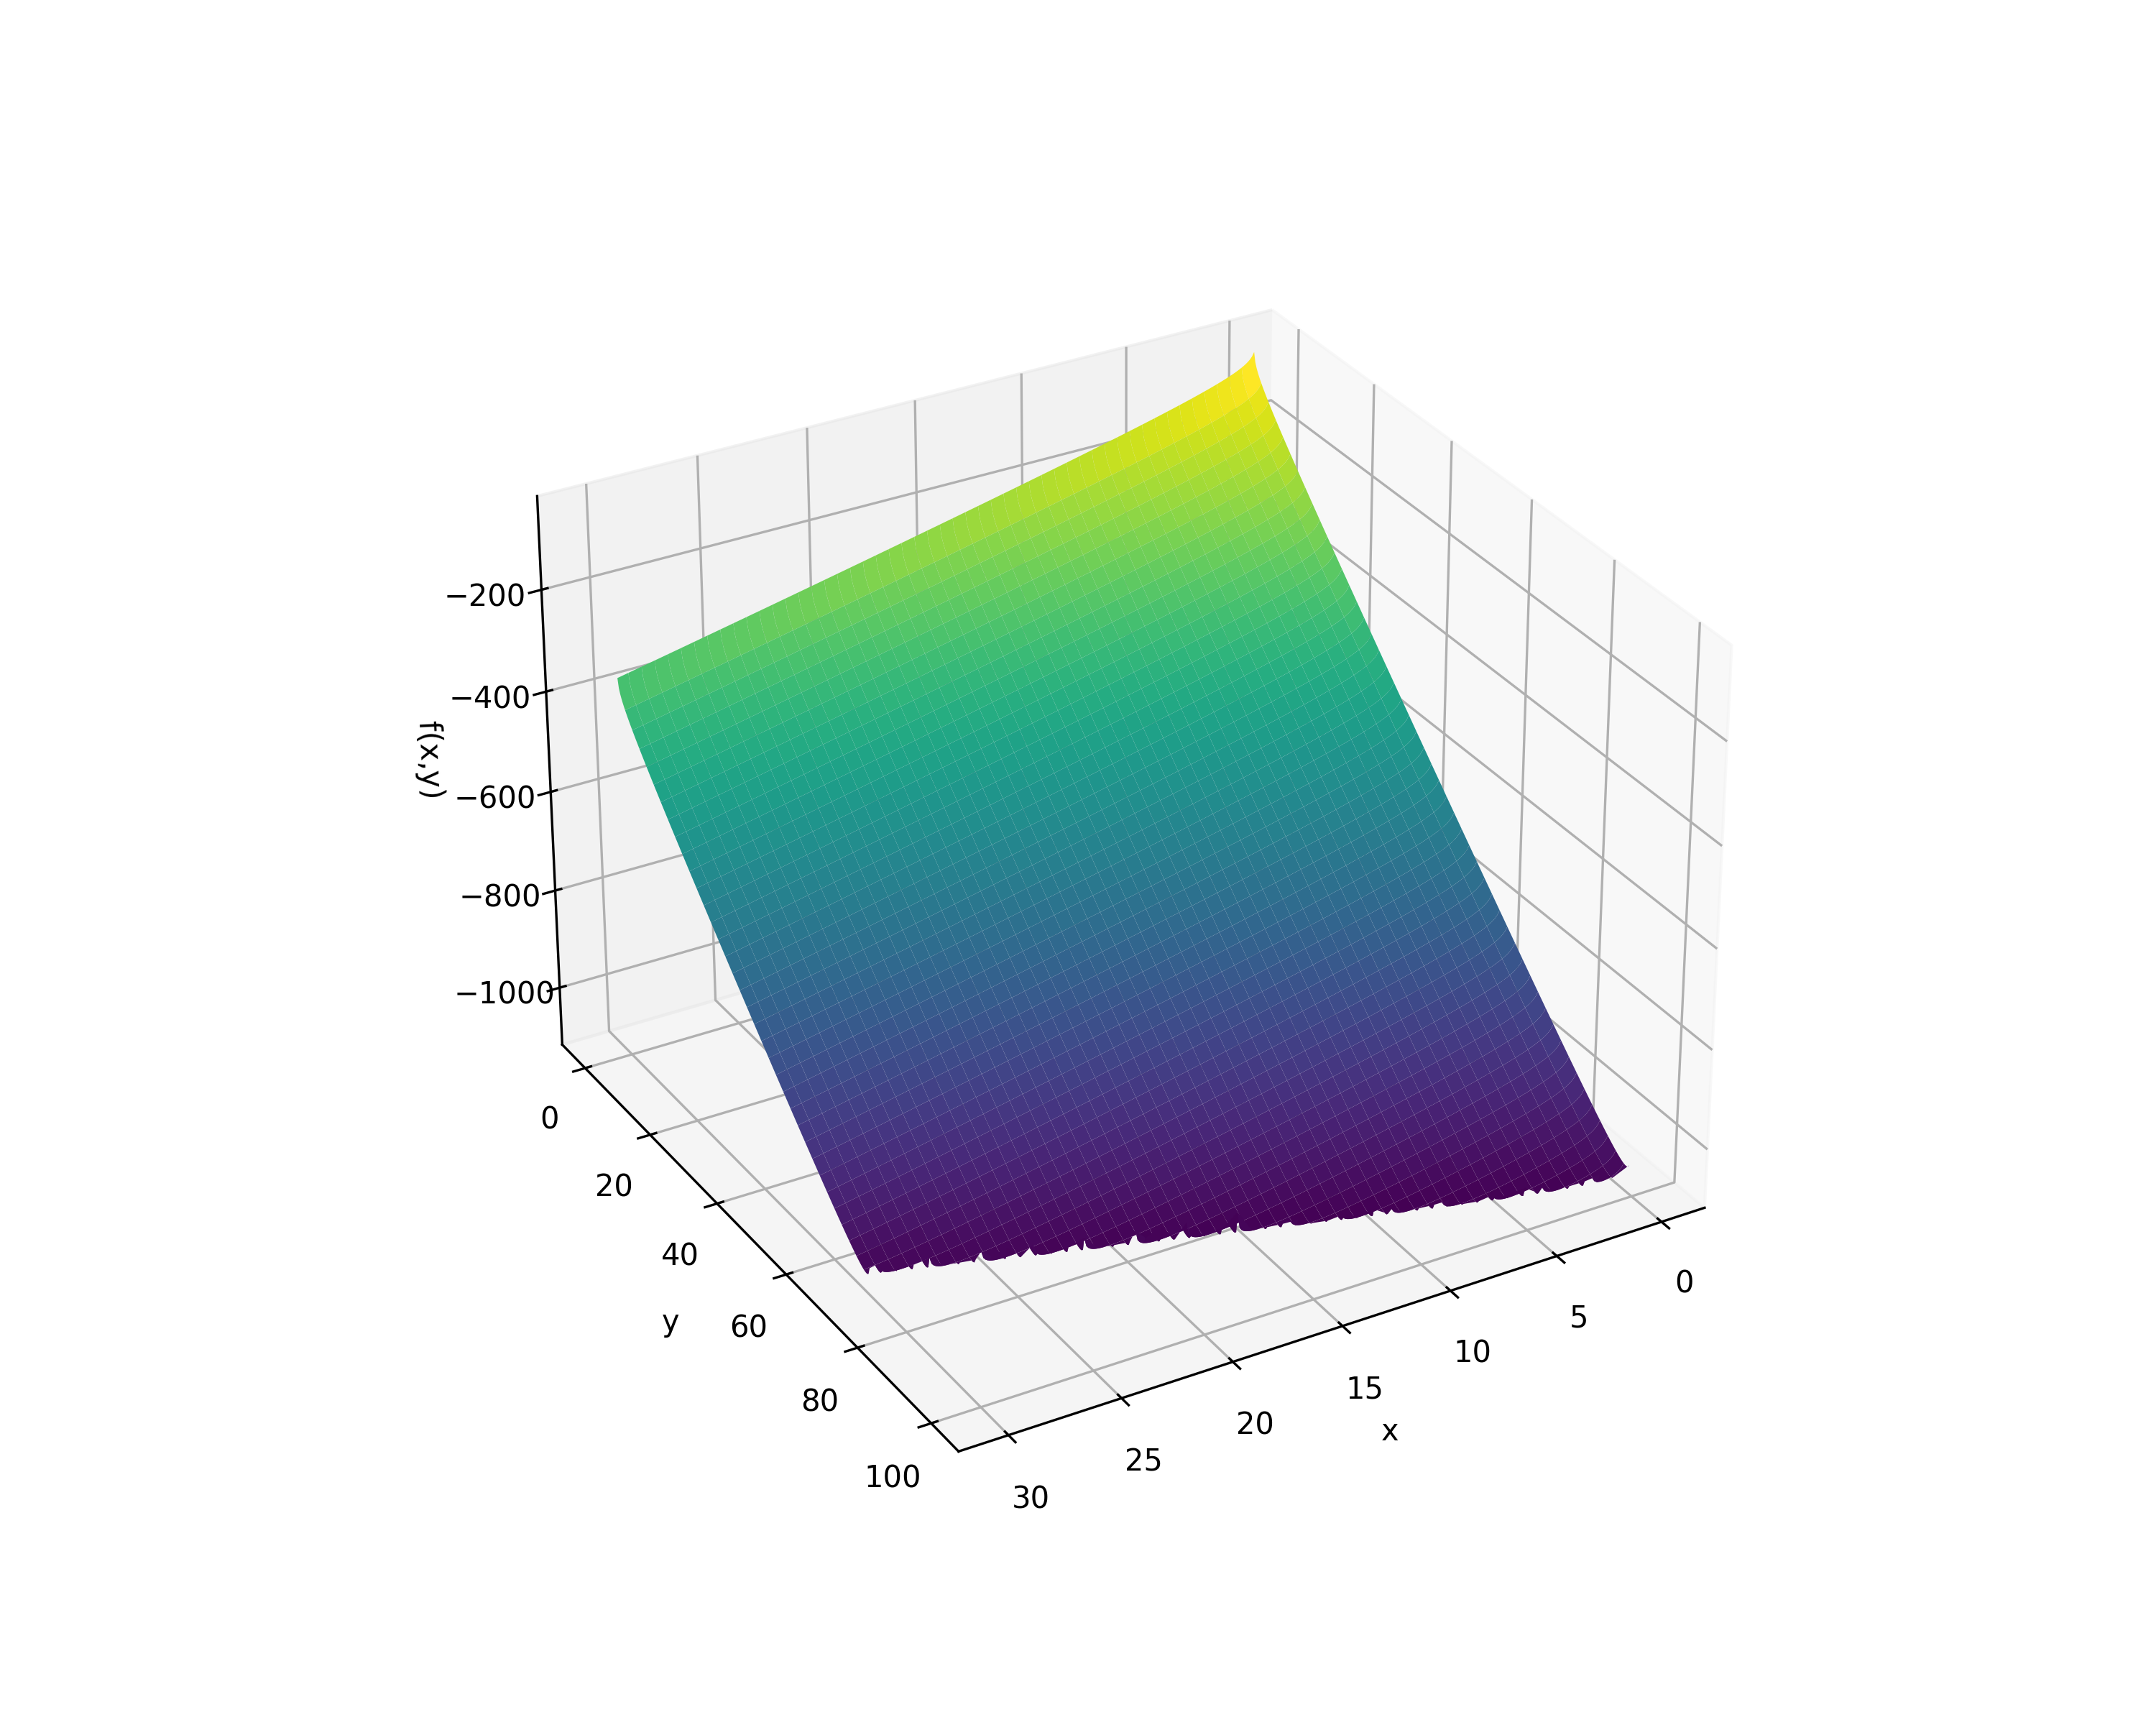
\includegraphics[width=\textwidth]{images/3d_function.png}
    \caption{3D-график функции.}
\end{figure}
\noindent На 3D-графике функция представлена в виде гладкой поверхности с четко выраженной областью определения (учитывая ограничения \(x>0\), \(y>0\), \(100-x-y>0\) и \(50-x+y>0\)). Цветовая схема иллюстрирует распределение значений функции: более темные оттенки соответствуют меньшим значениям \(f(x,y)\). График показывает наличие локального минимума, что служит отправной точкой для дальнейшего применения метода Ньютона.

\begin{figure}[H]
    \centering
    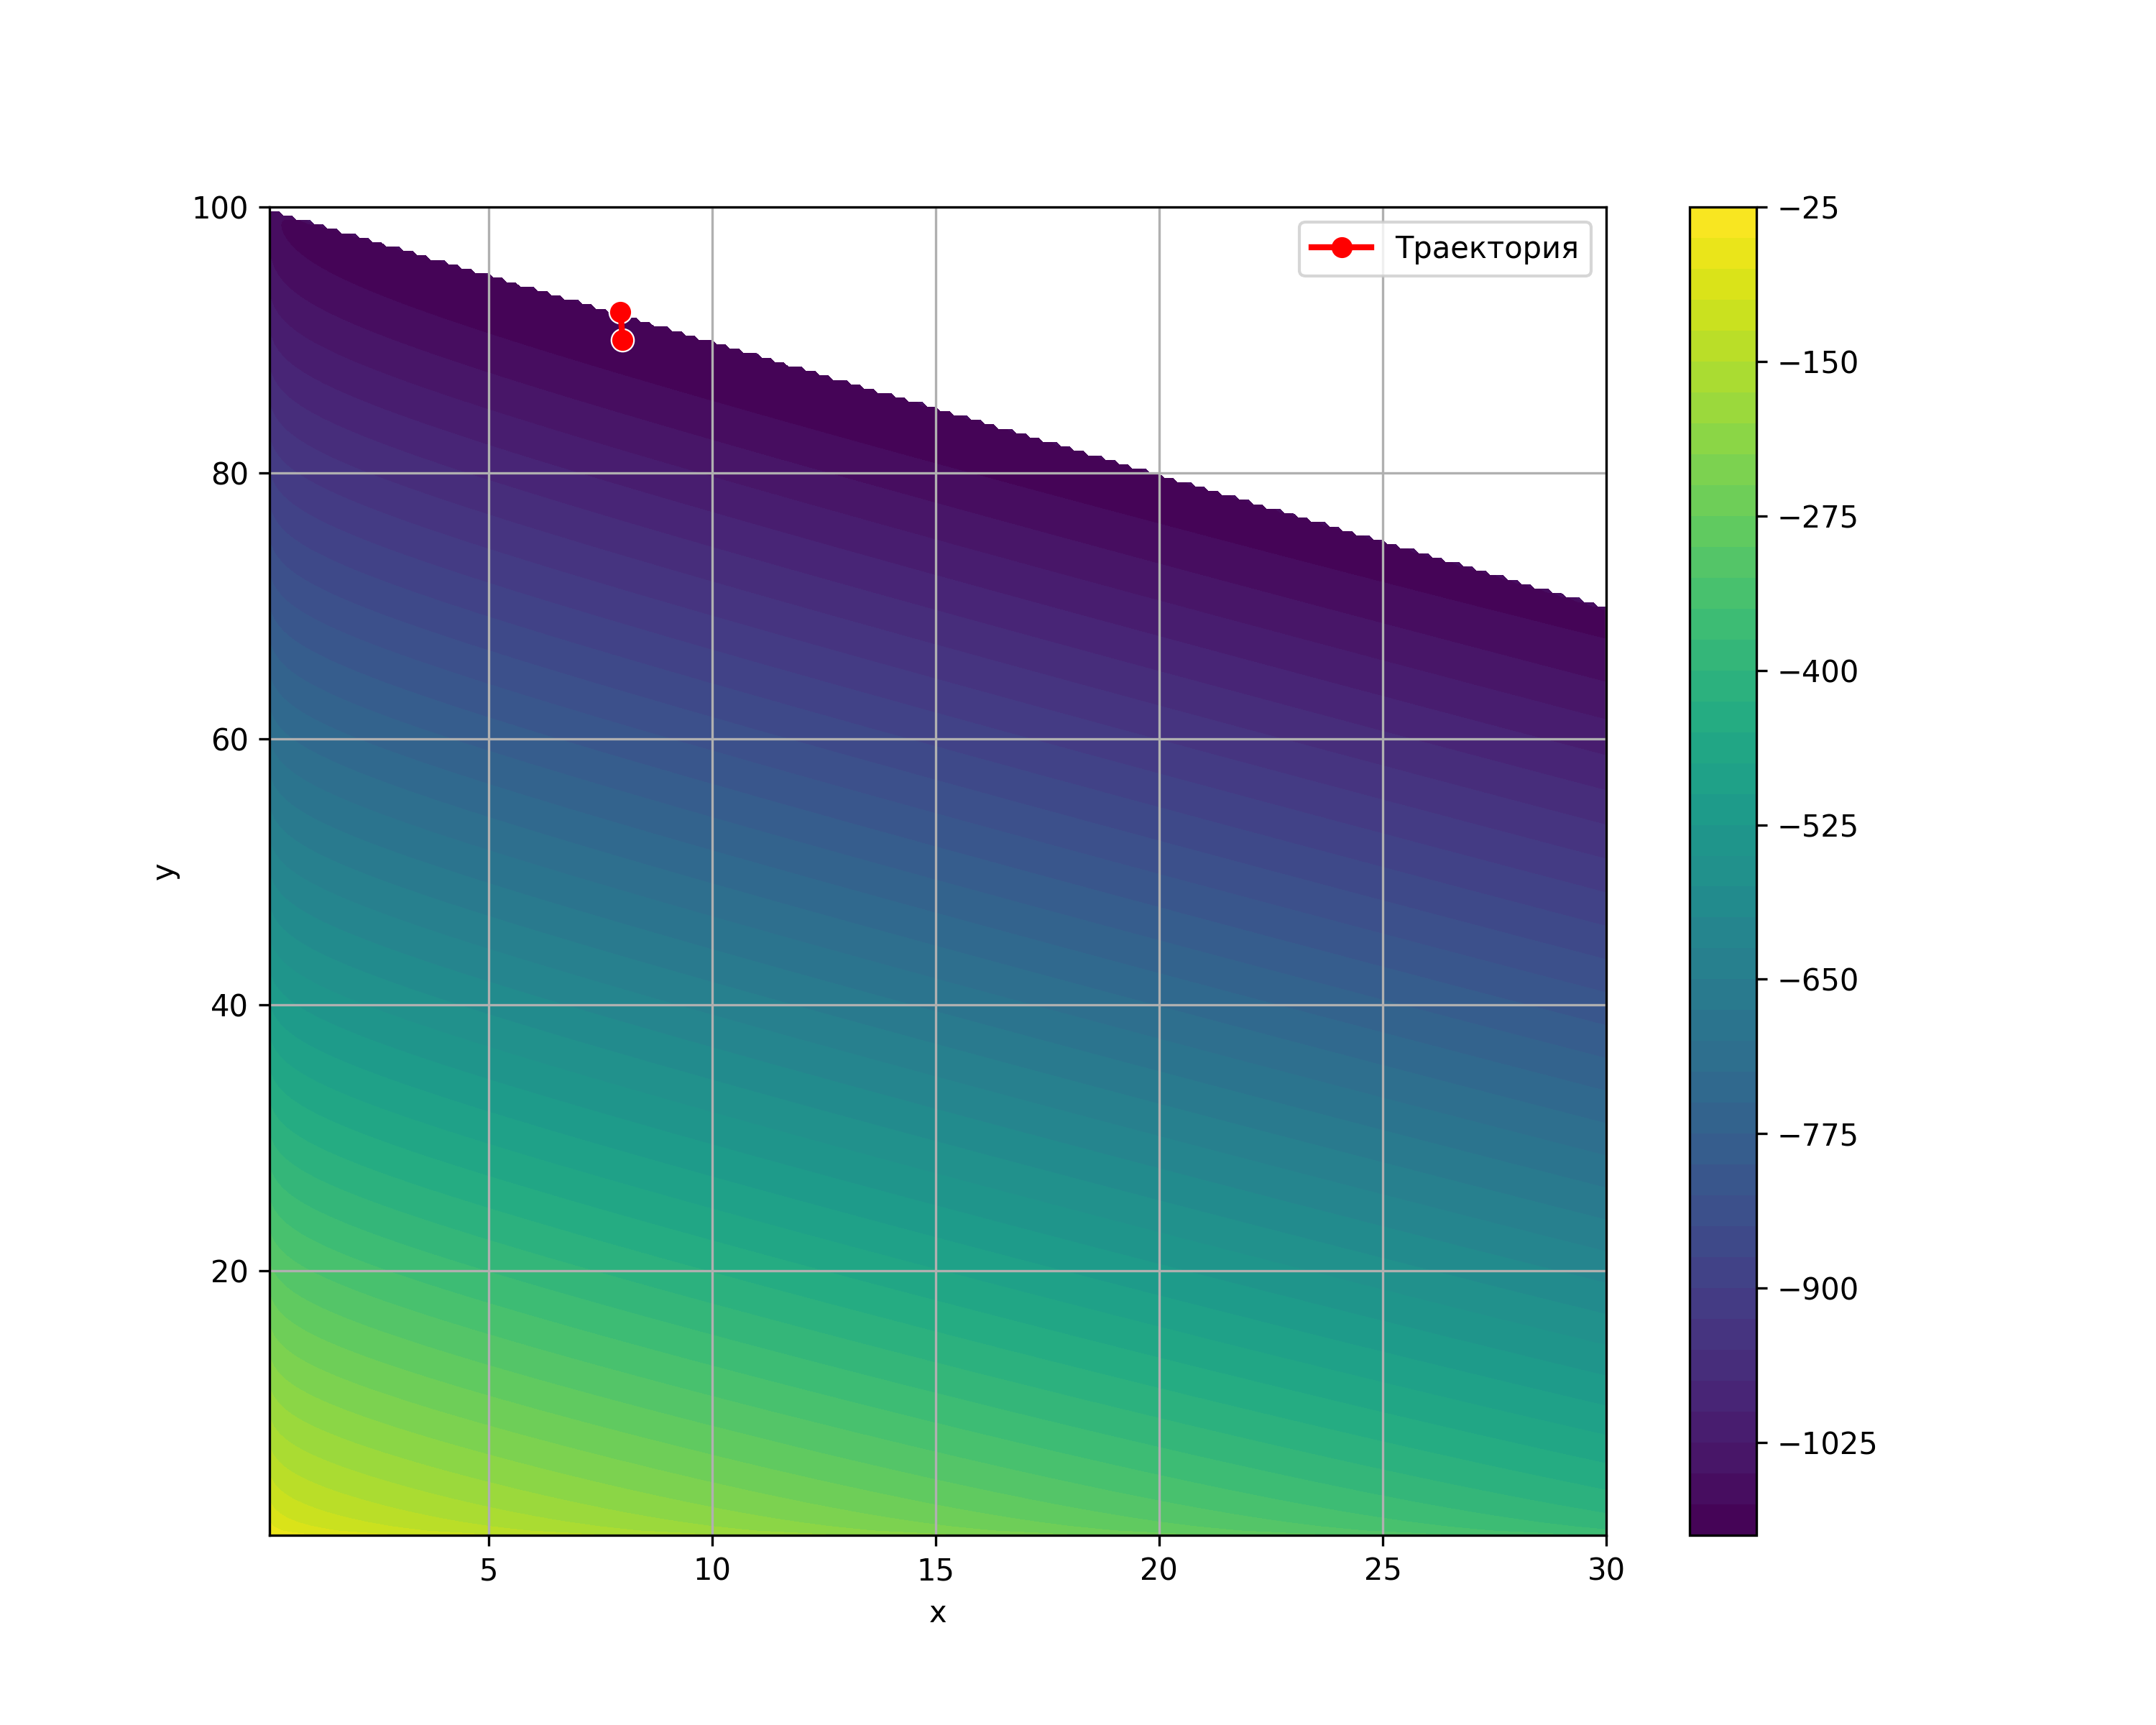
\includegraphics[width=0.49\textwidth]{images/newton_fixed_trajectory_0.png}
    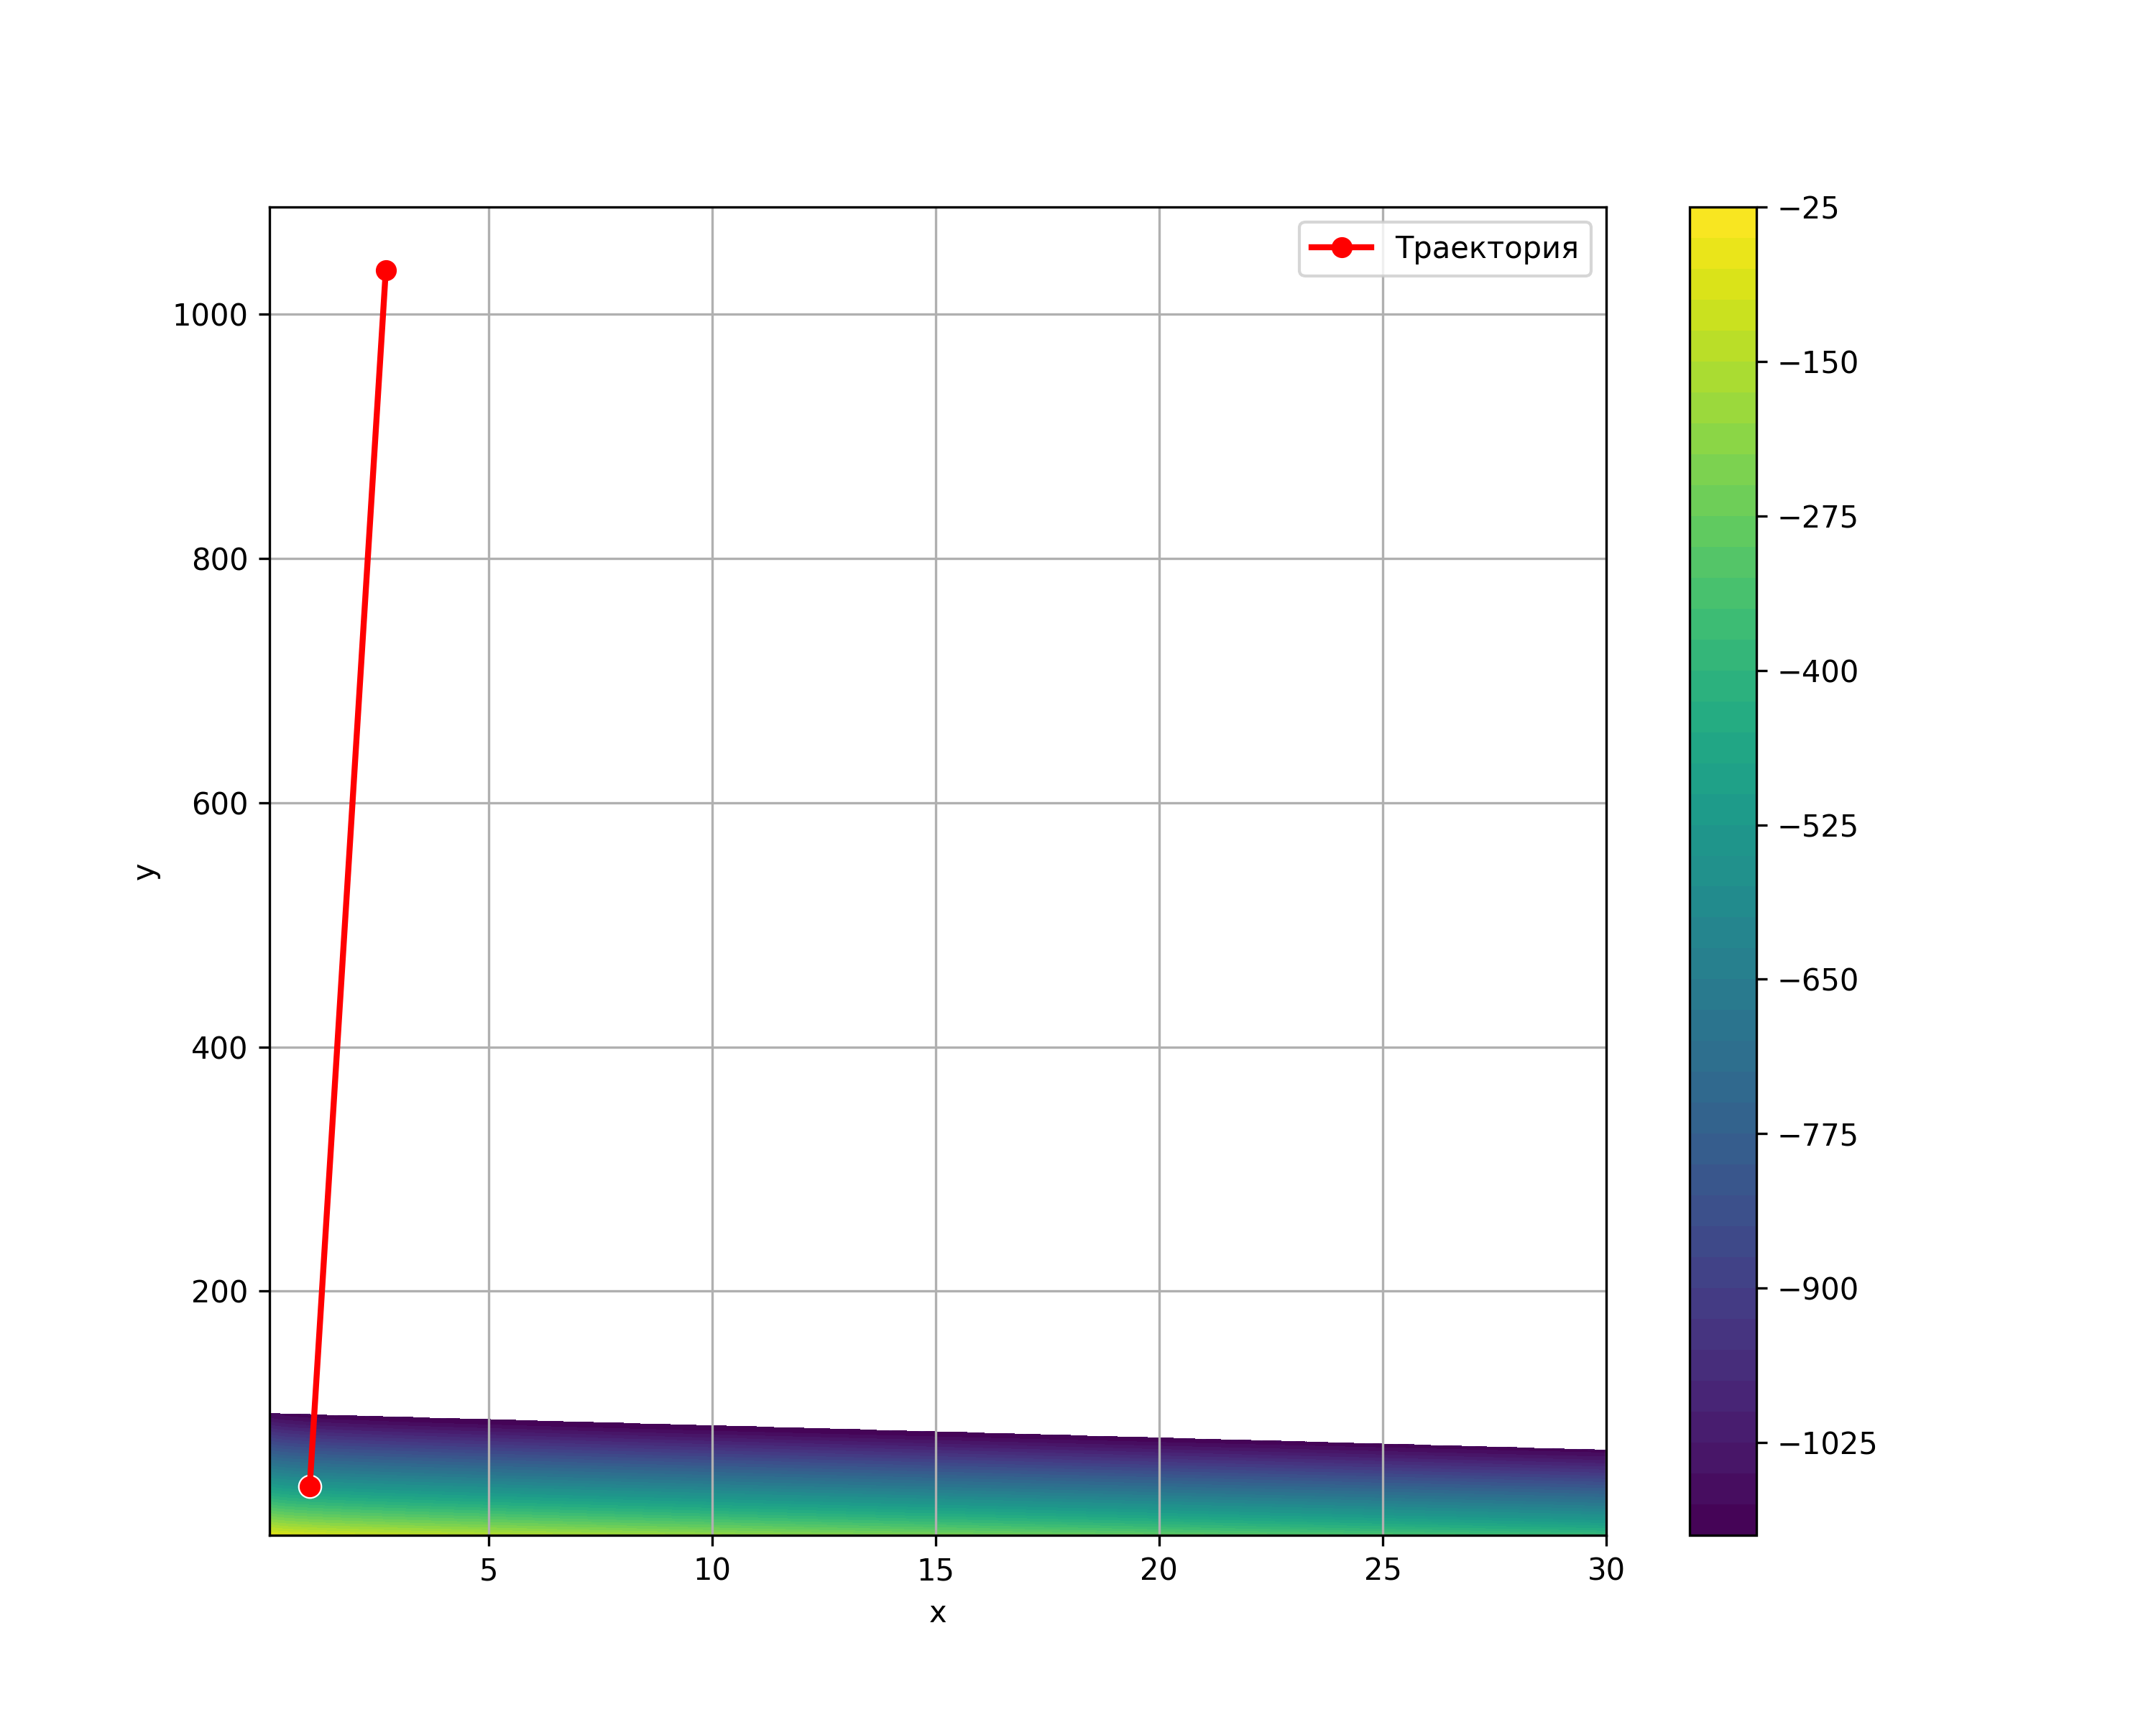
\includegraphics[width=0.49\textwidth]{images/newton_fixed_trajectory_1.png}
    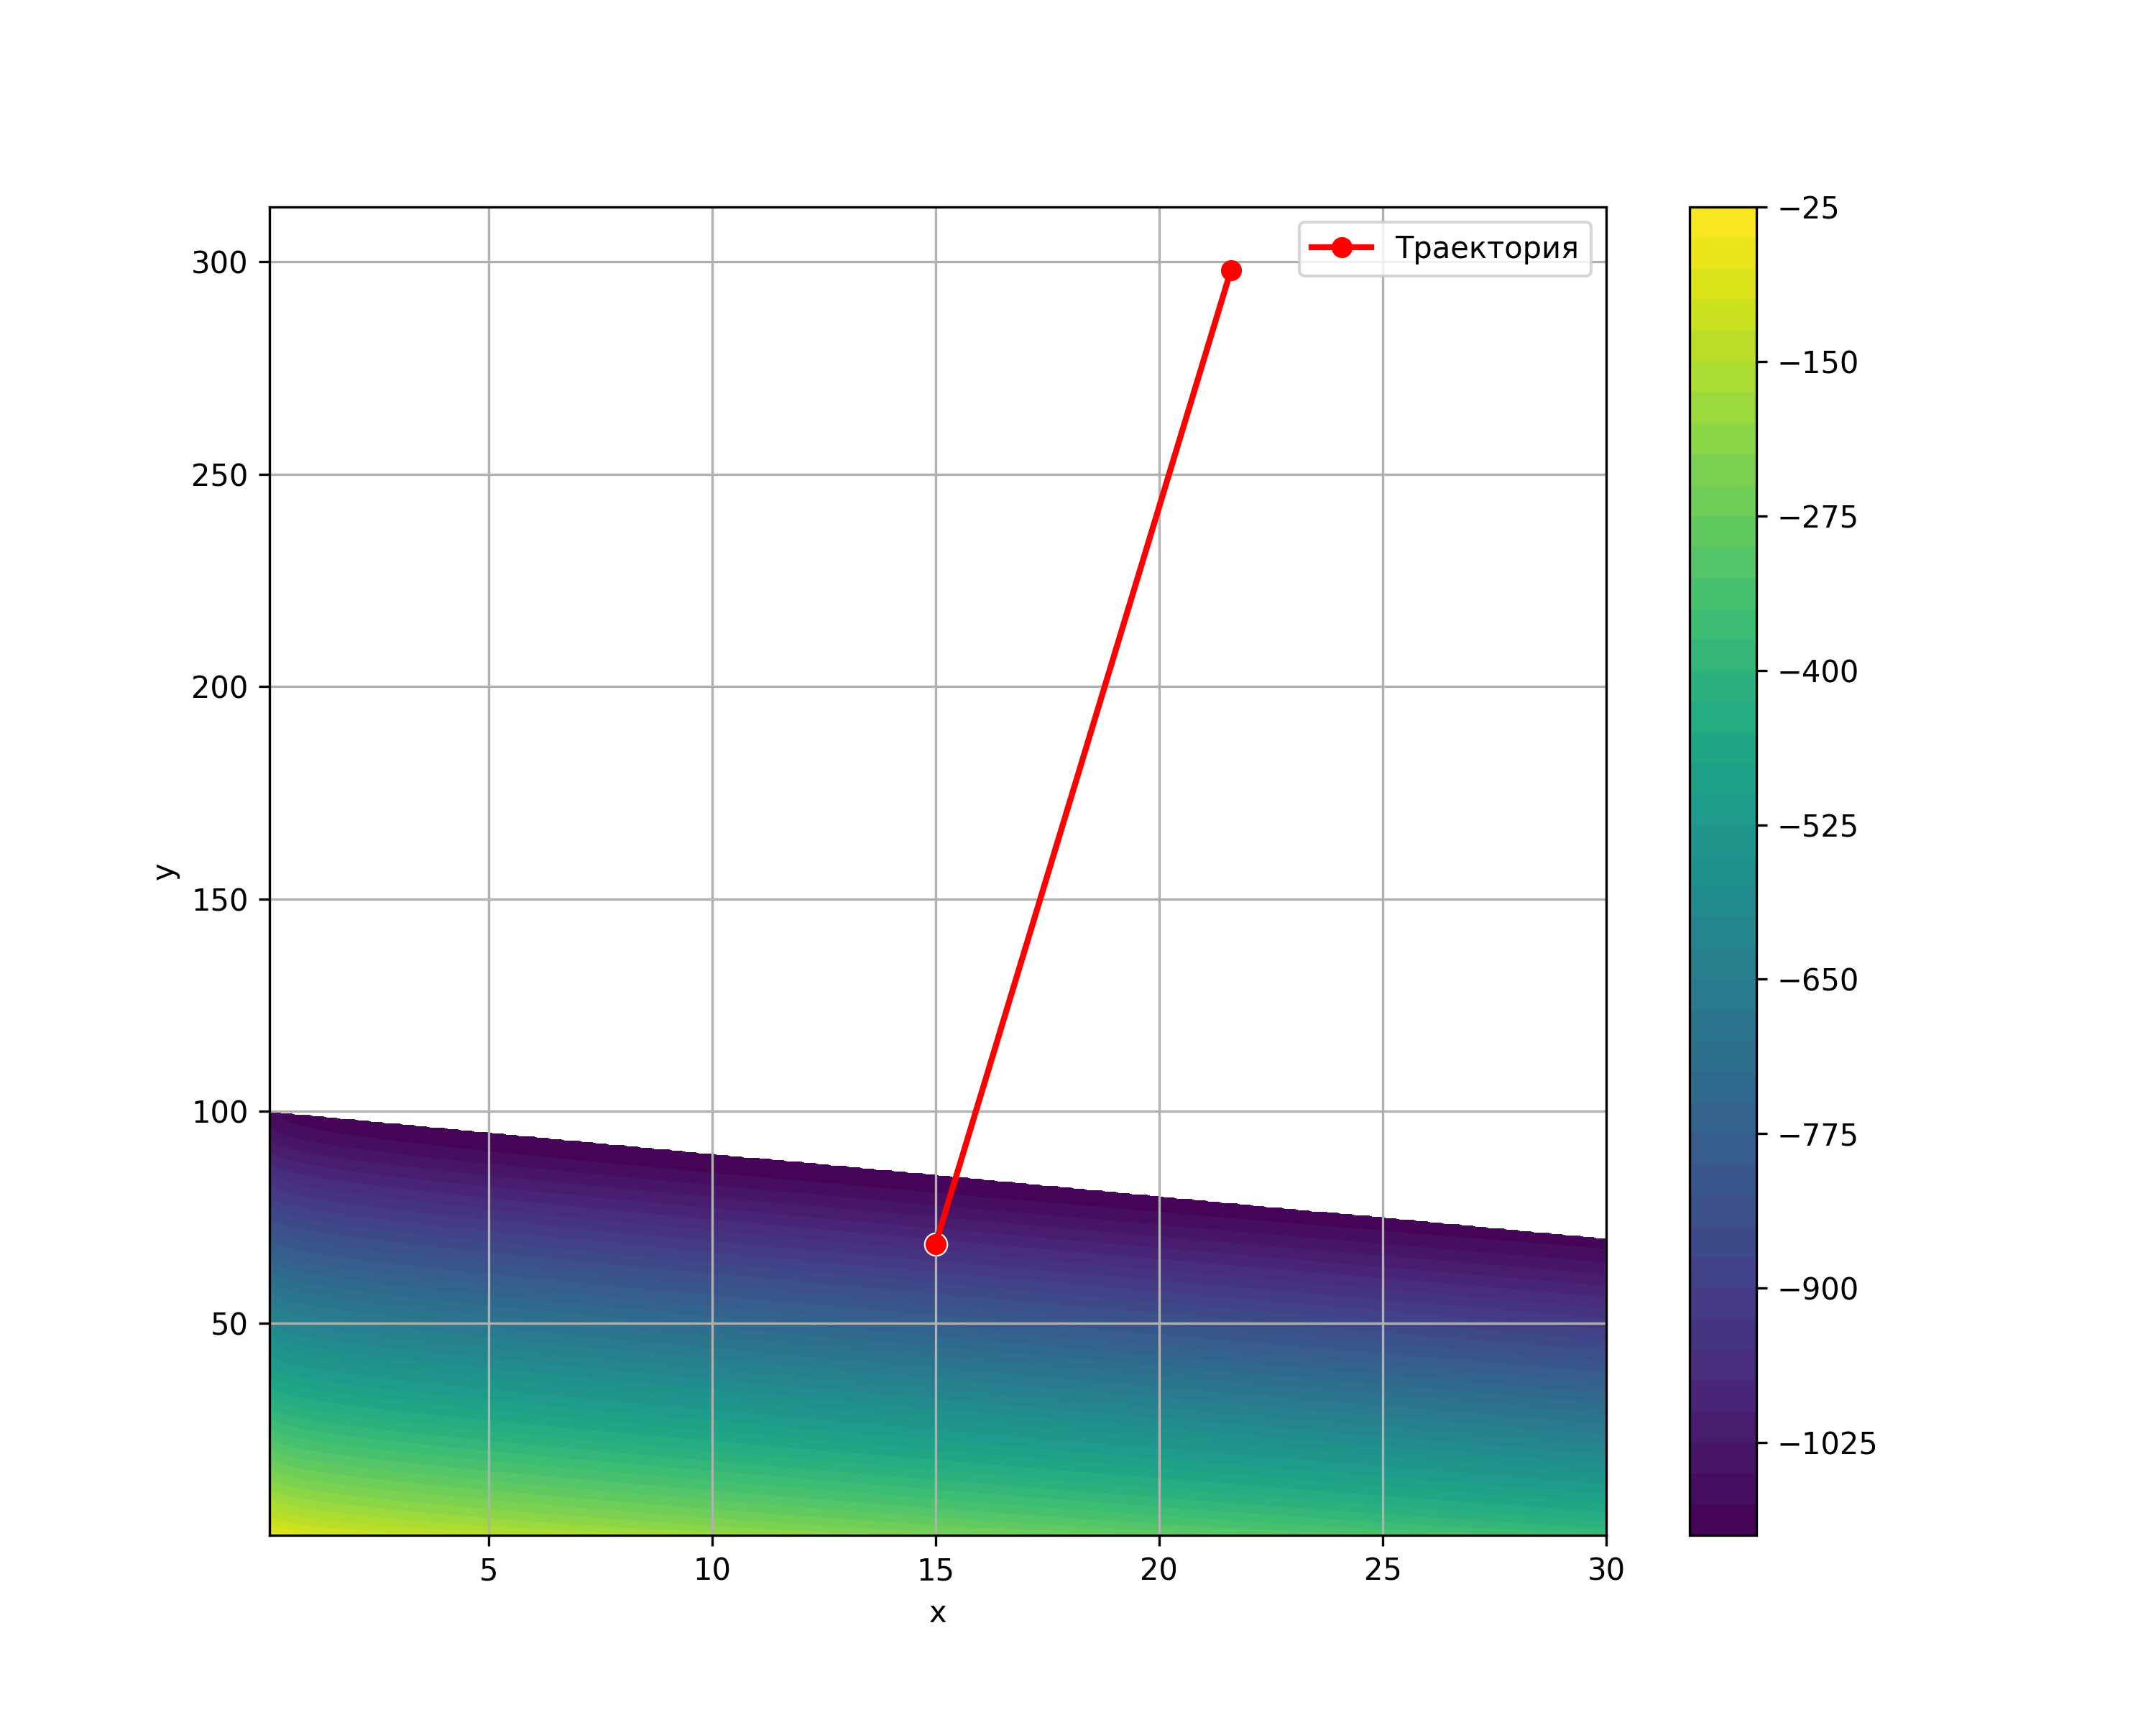
\includegraphics[width=0.49\textwidth]{images/newton_fixed_trajectory_2.png}
    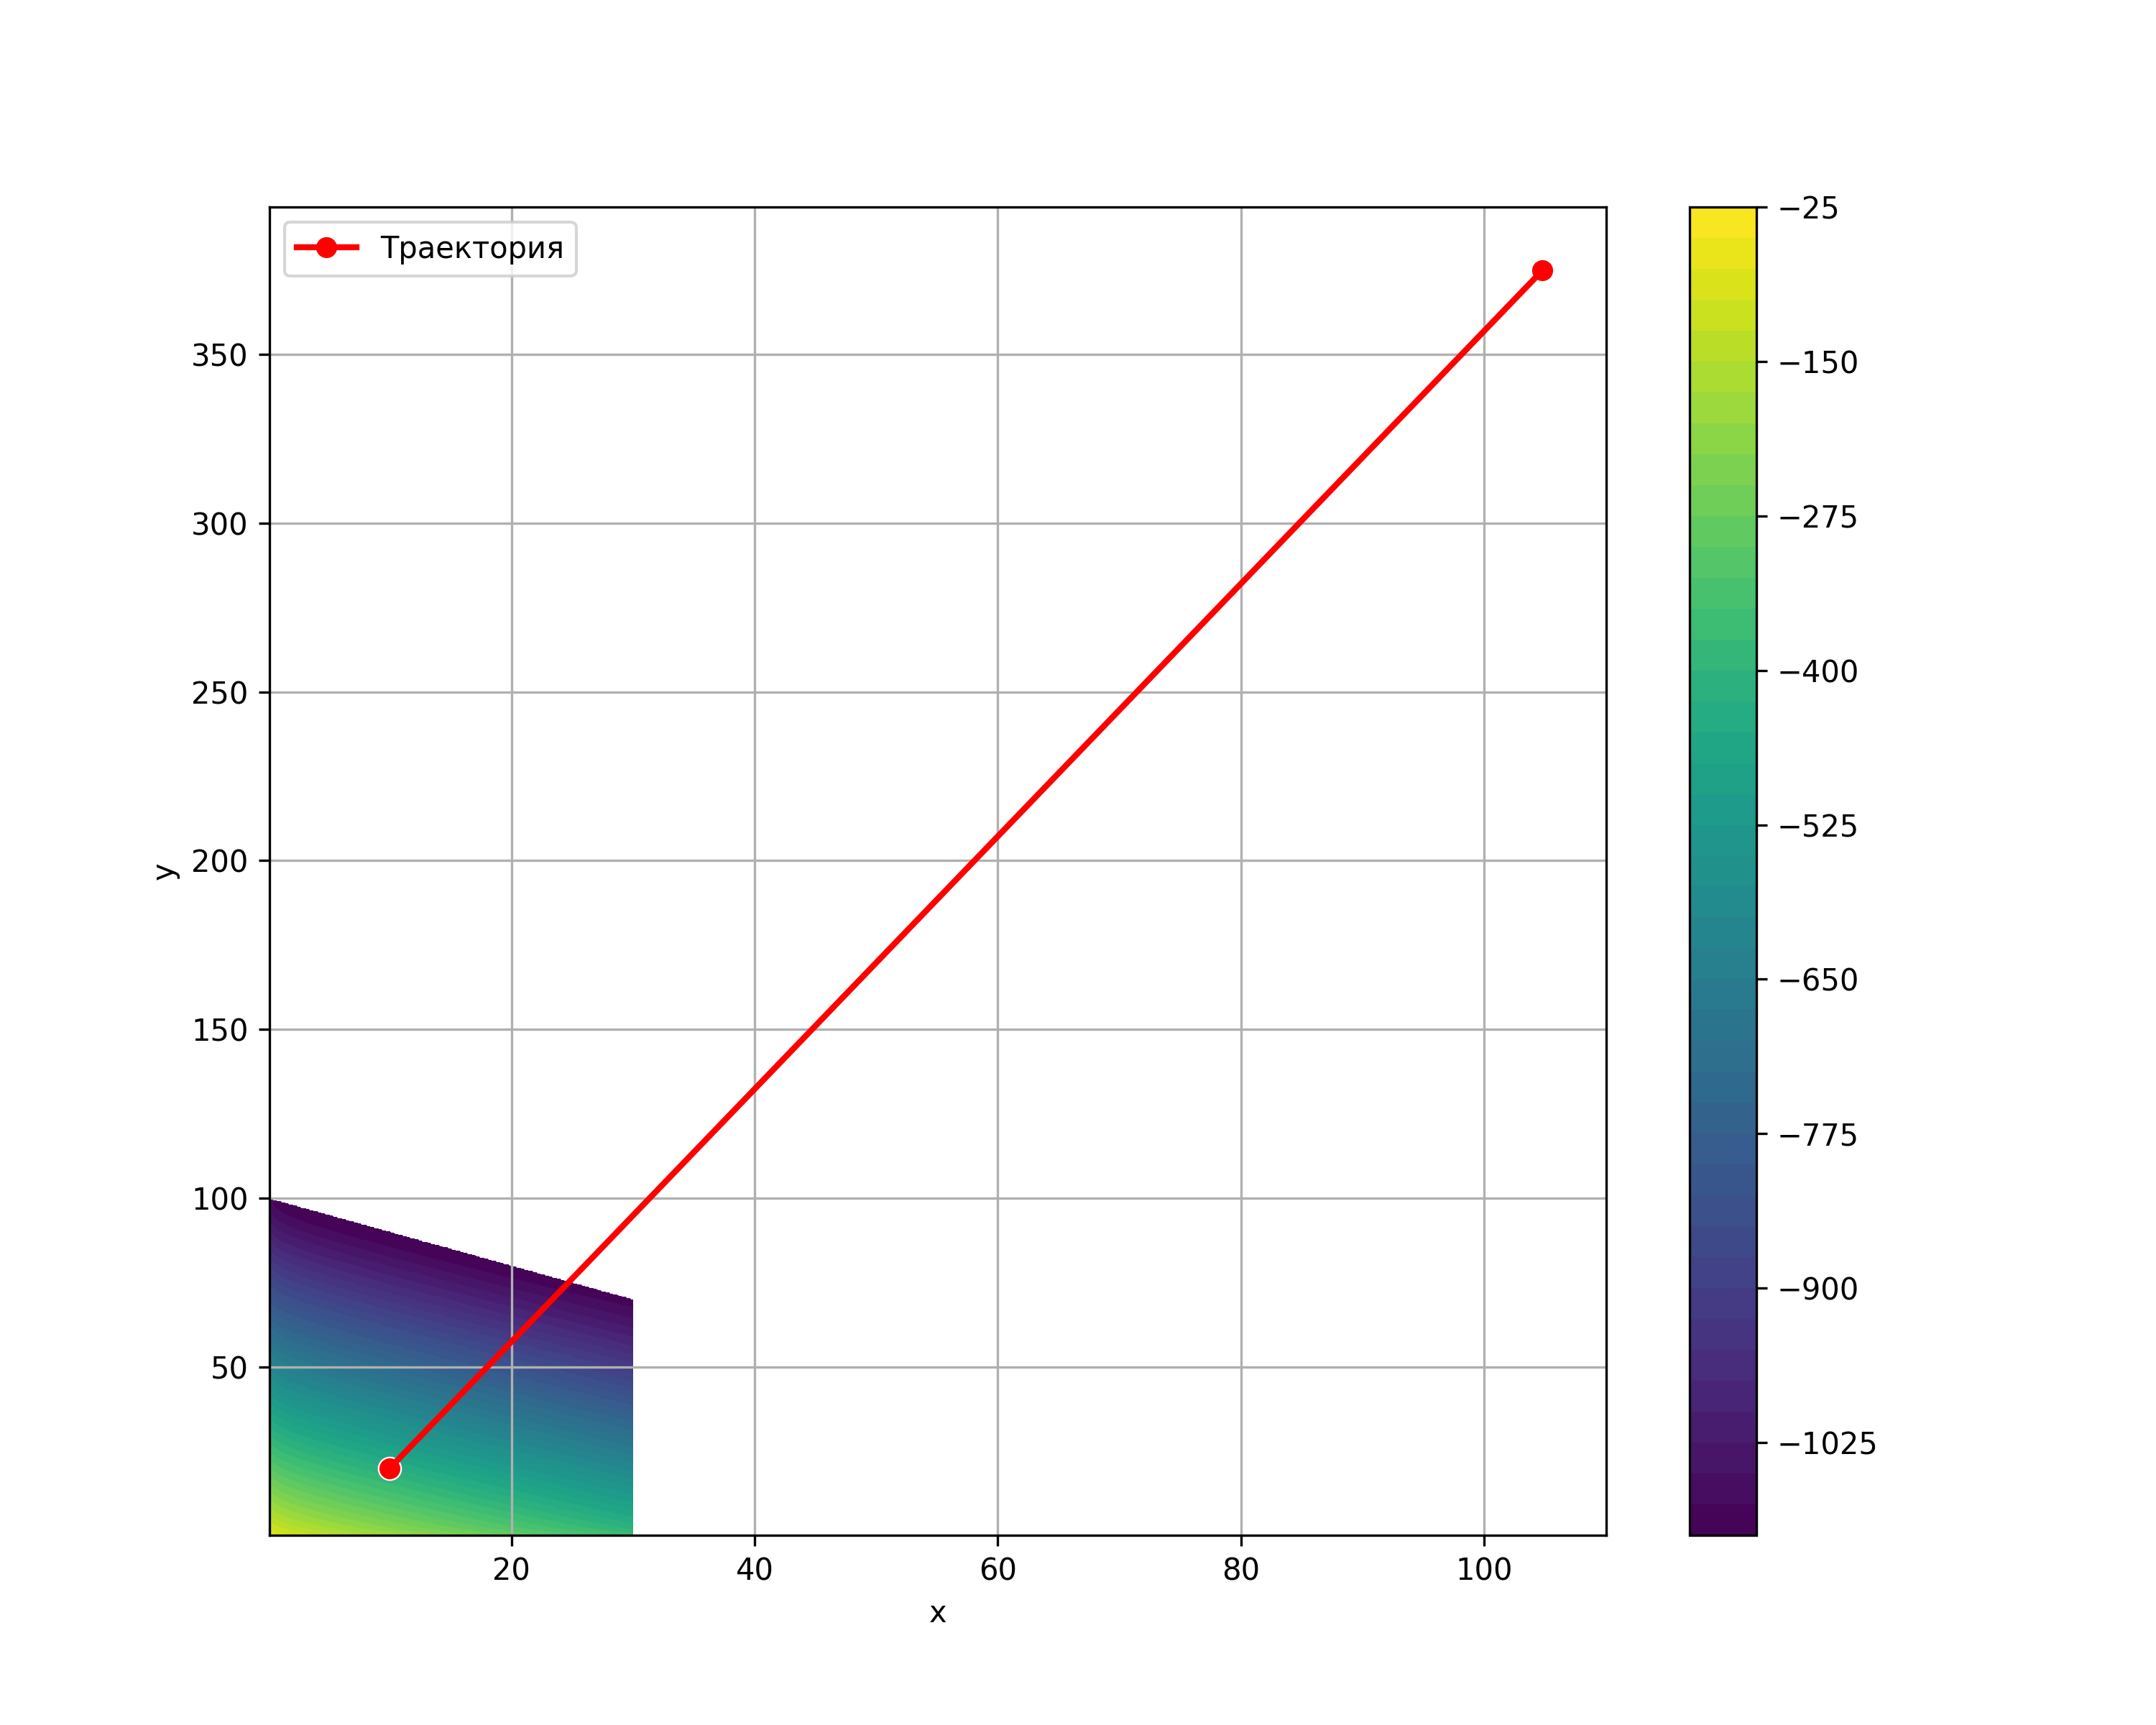
\includegraphics[width=0.49\textwidth]{images/newton_fixed_trajectory_3.png}
    \caption{Траектории итераций метода Ньютона с фиксированным шагом \(\alpha=1\) для различных начальных точек.}
\end{figure}
\noindent При использовании фиксированного шага \(\alpha=1\) наблюдается, что итерационный процесс, не учитывая ограничения области определения функции, приводит к тому, что точки итераций <<улетают в космос>> – выходят за пределы допустимой области.

\begin{figure}[H]
    \centering 
    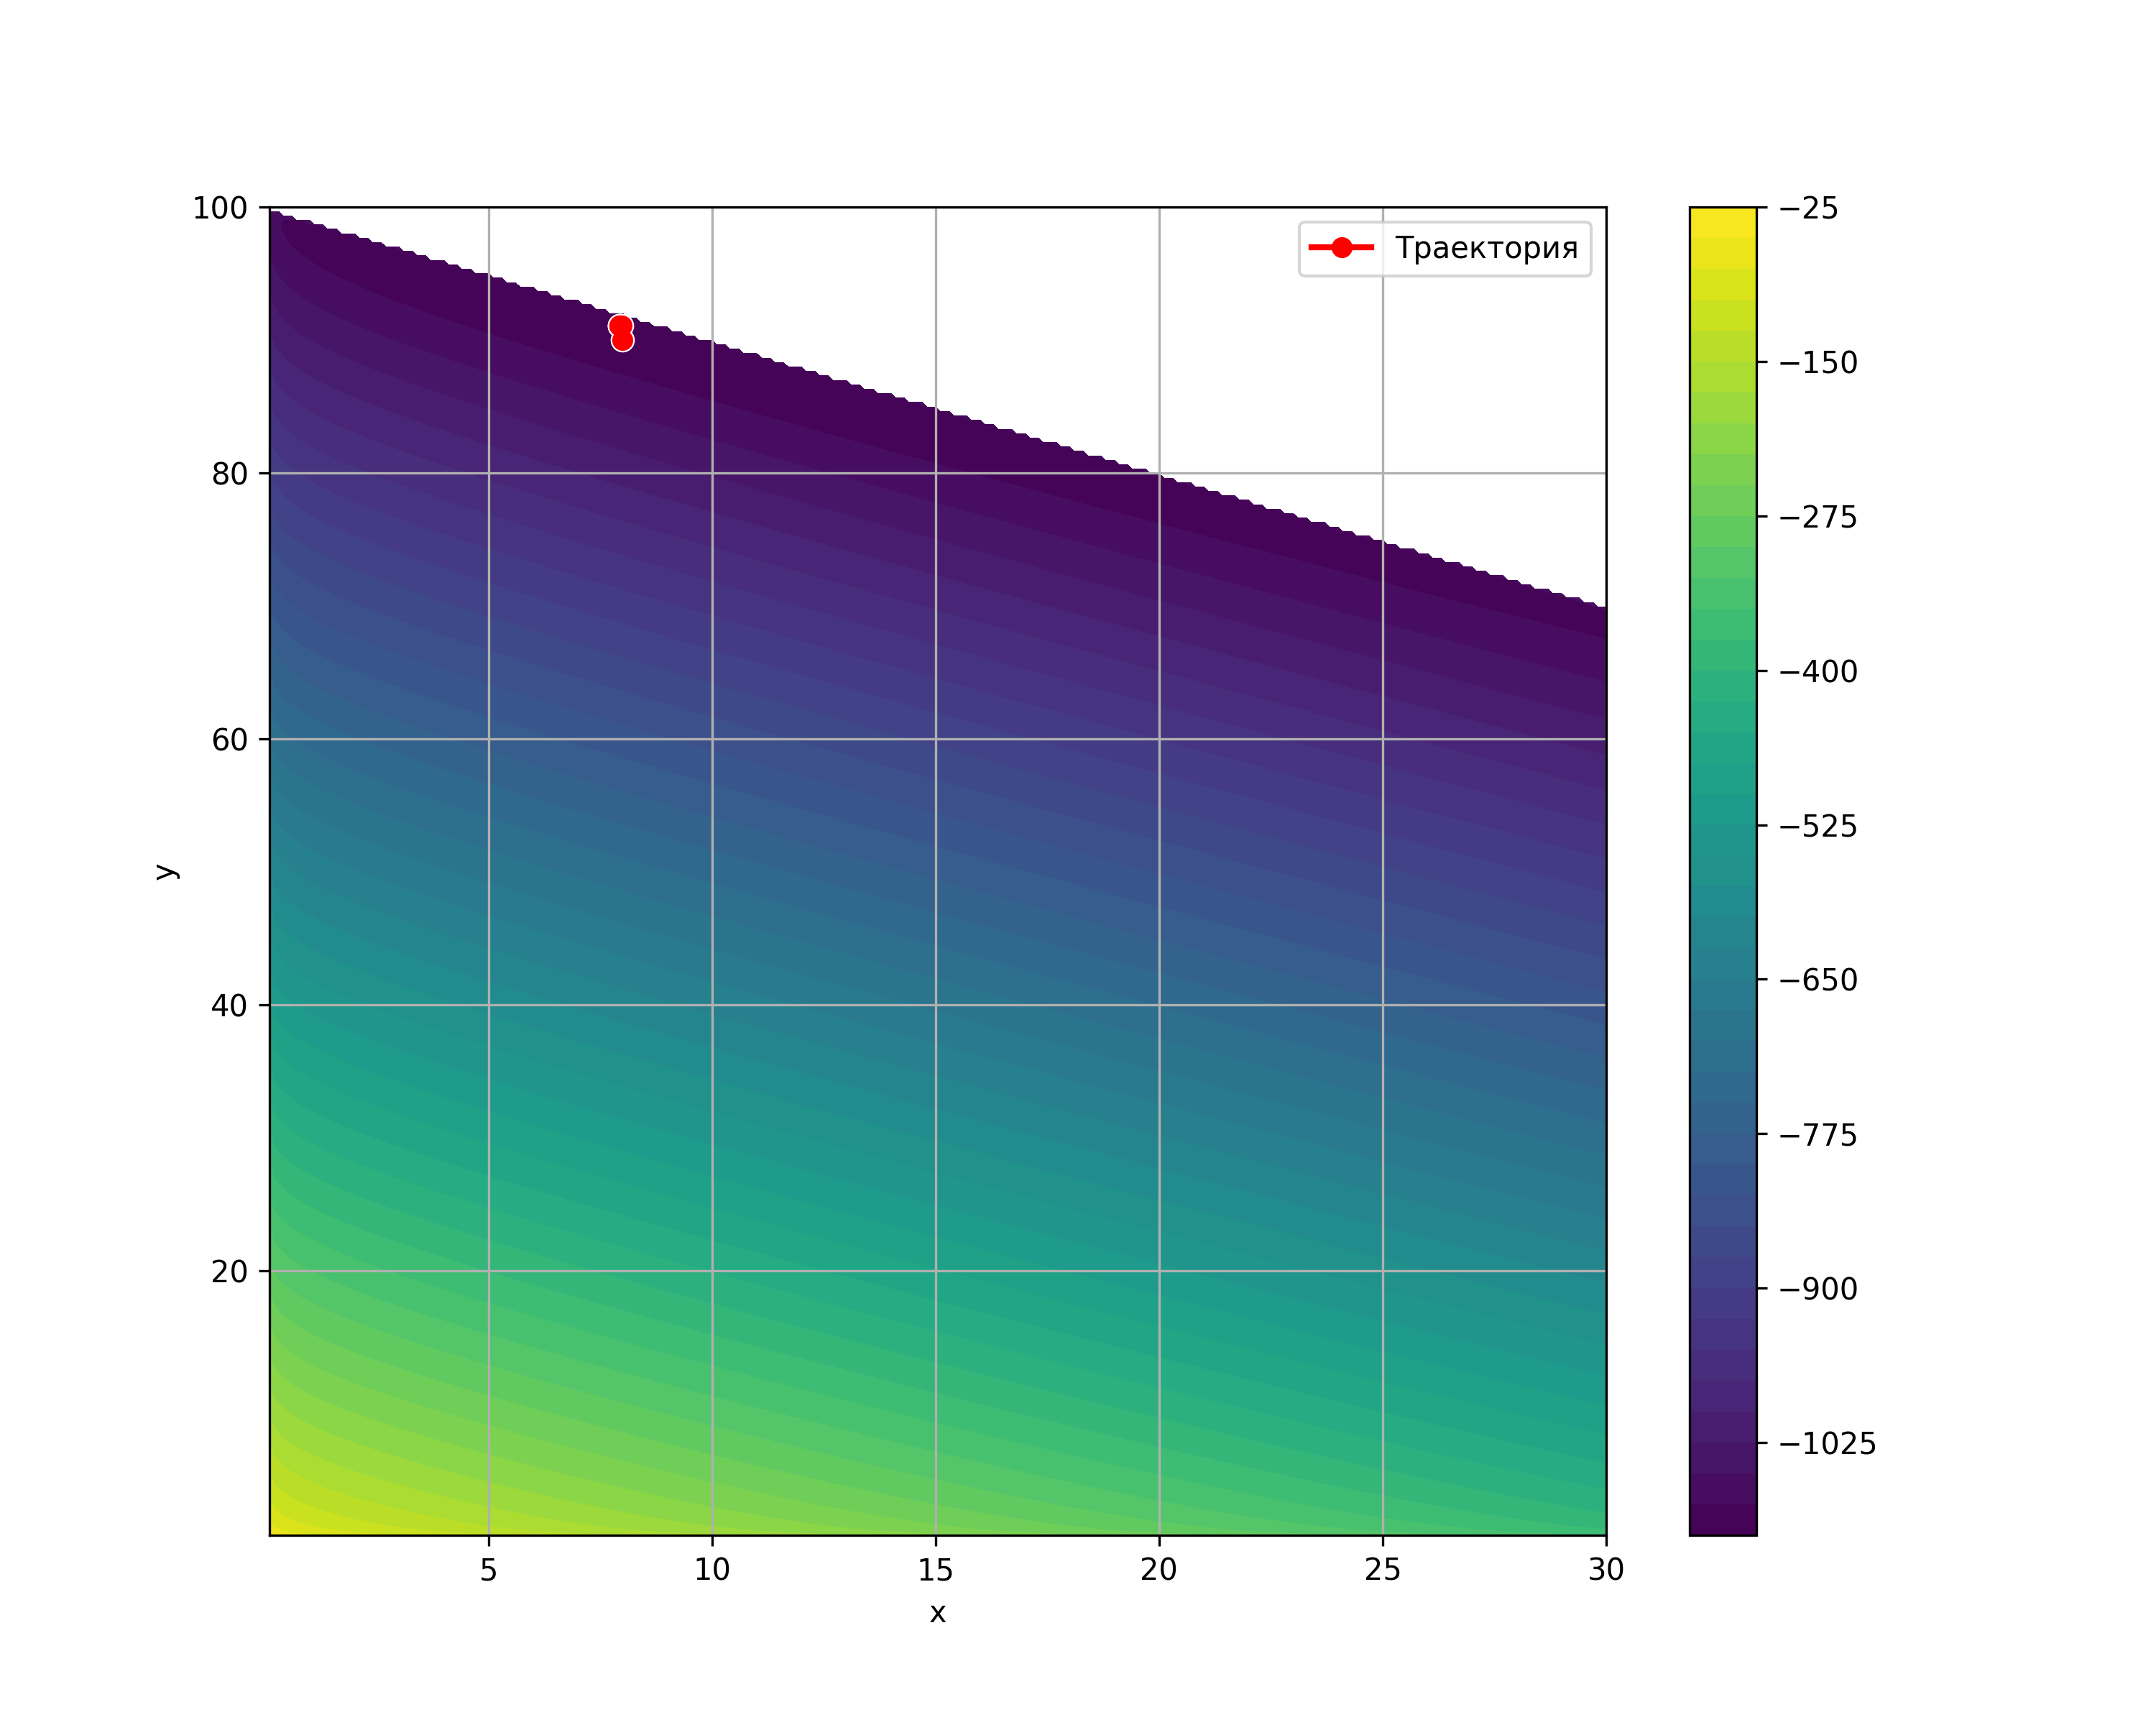
\includegraphics[width=0.49\textwidth]{images/newton_adaptive_trajectory_0.png}
    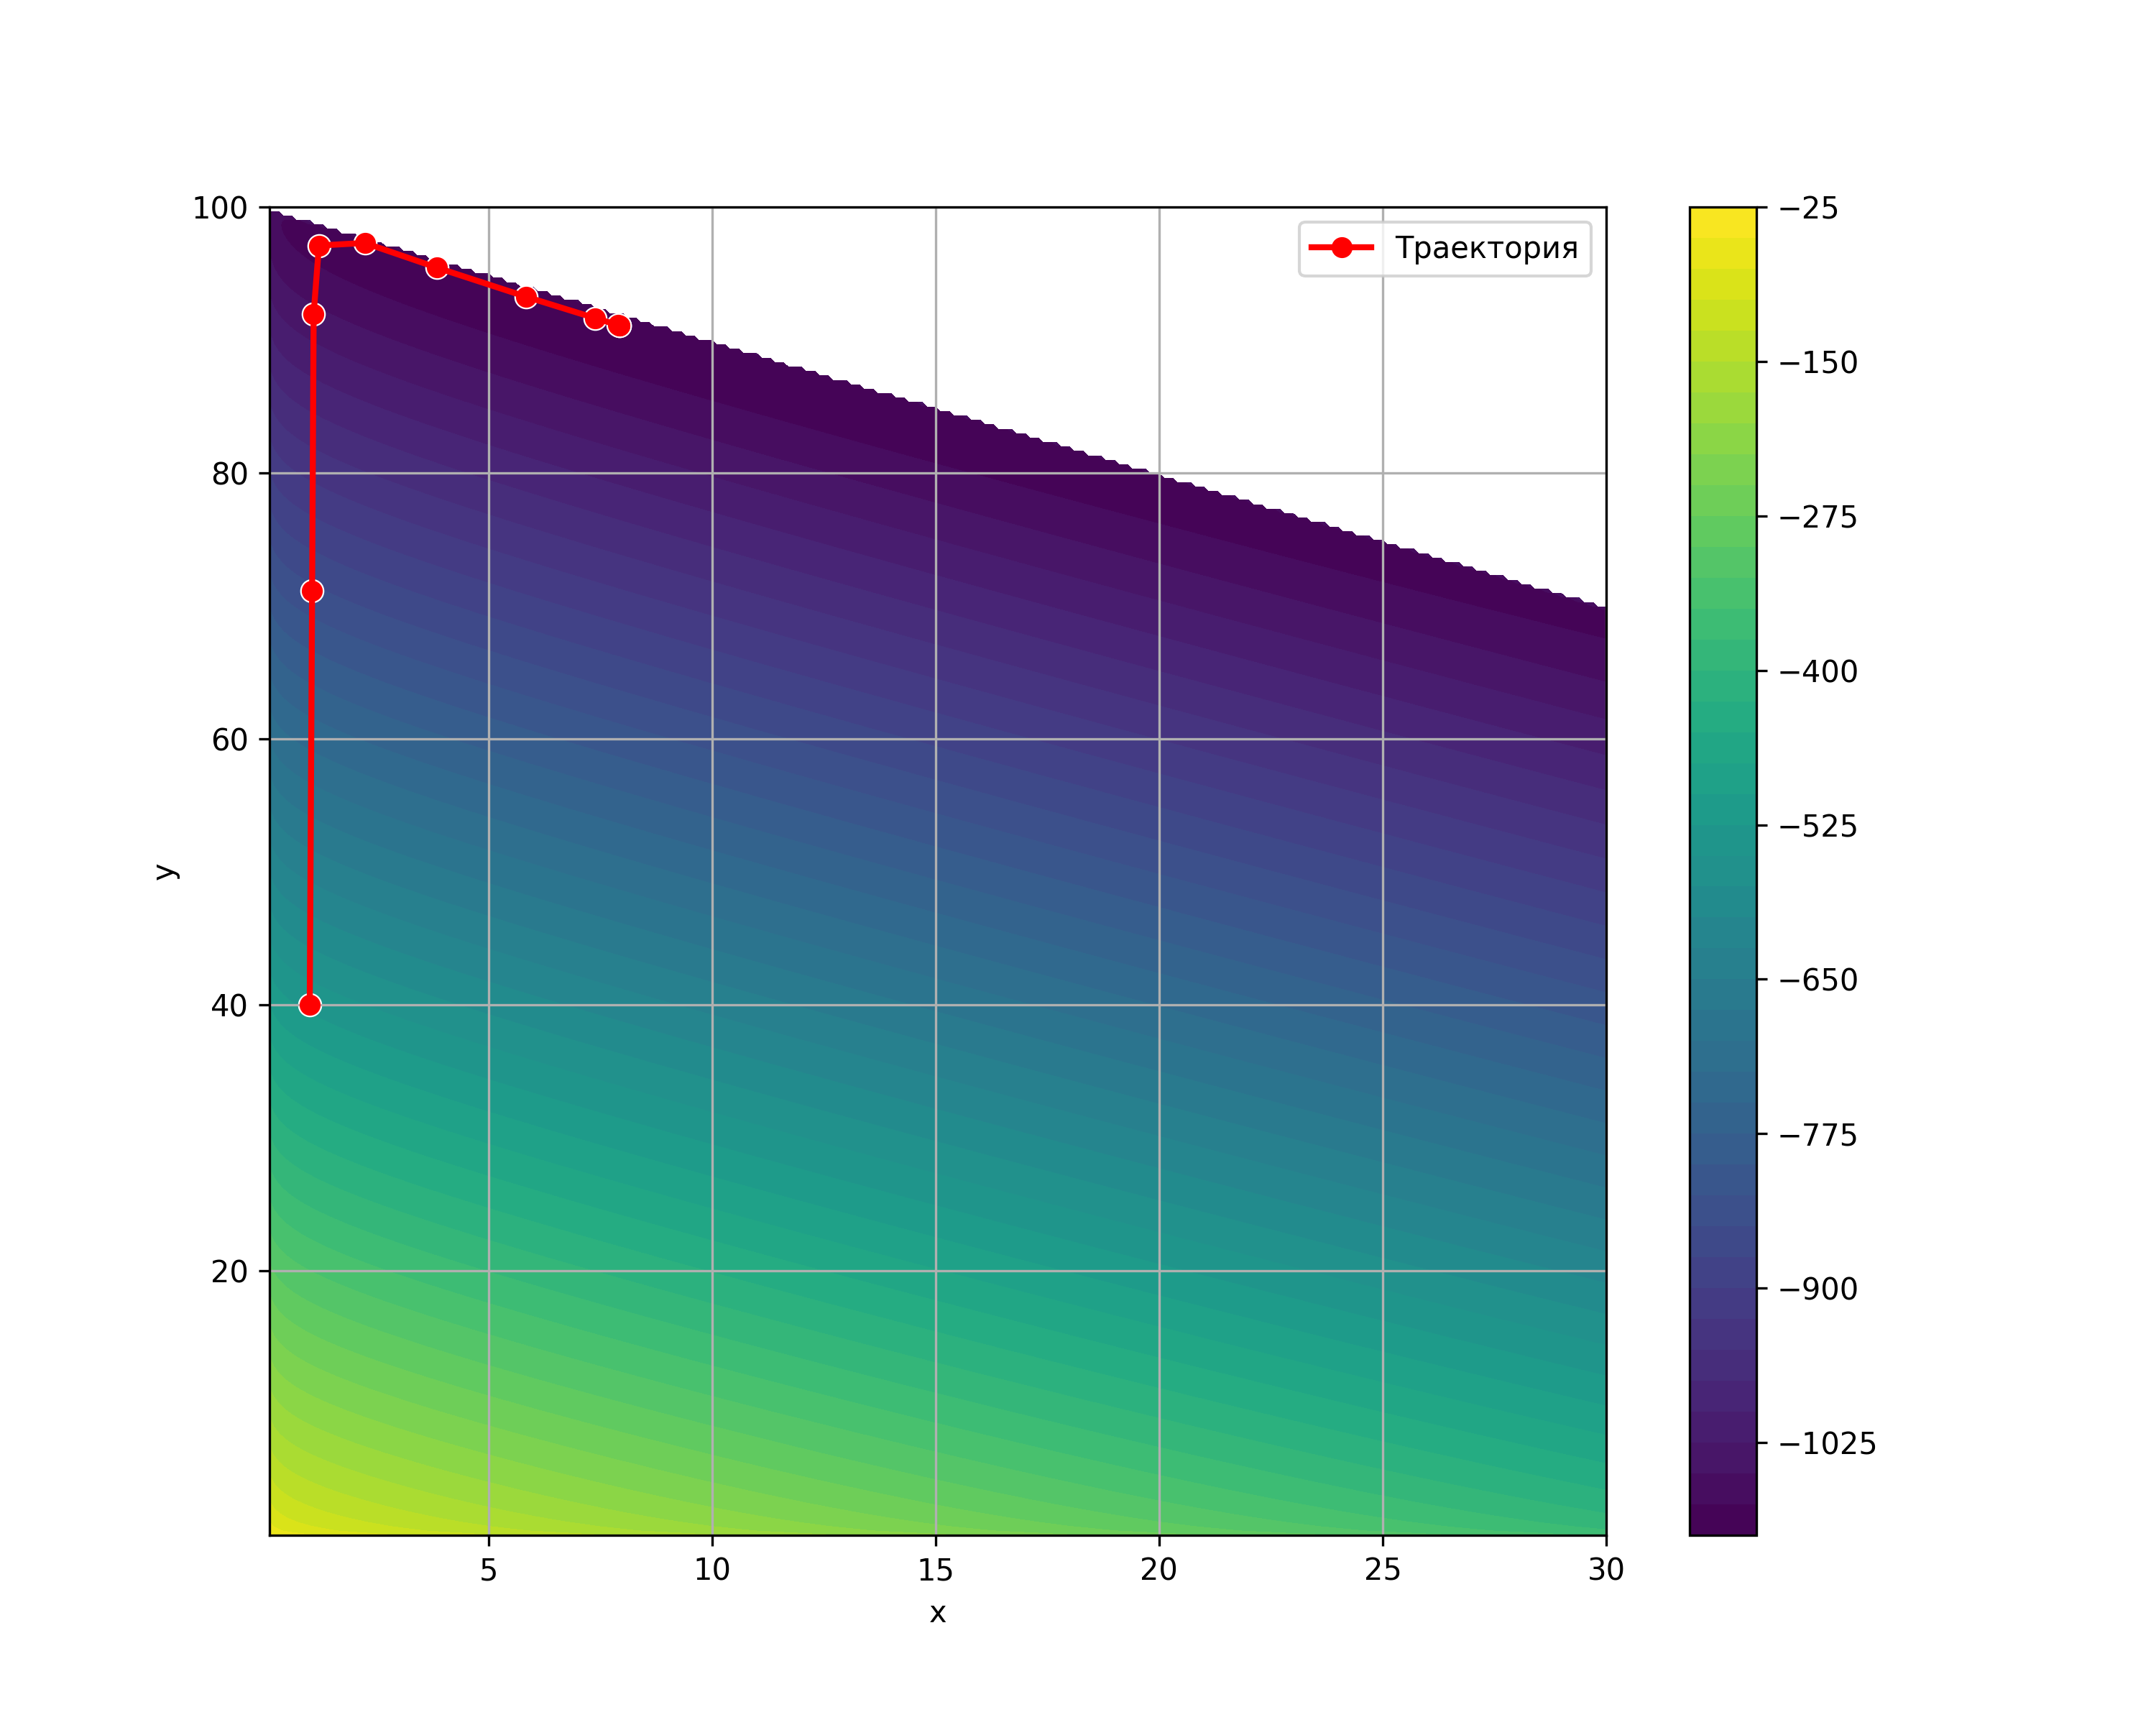
\includegraphics[width=0.49\textwidth]{images/newton_adaptive_trajectory_1.png}
    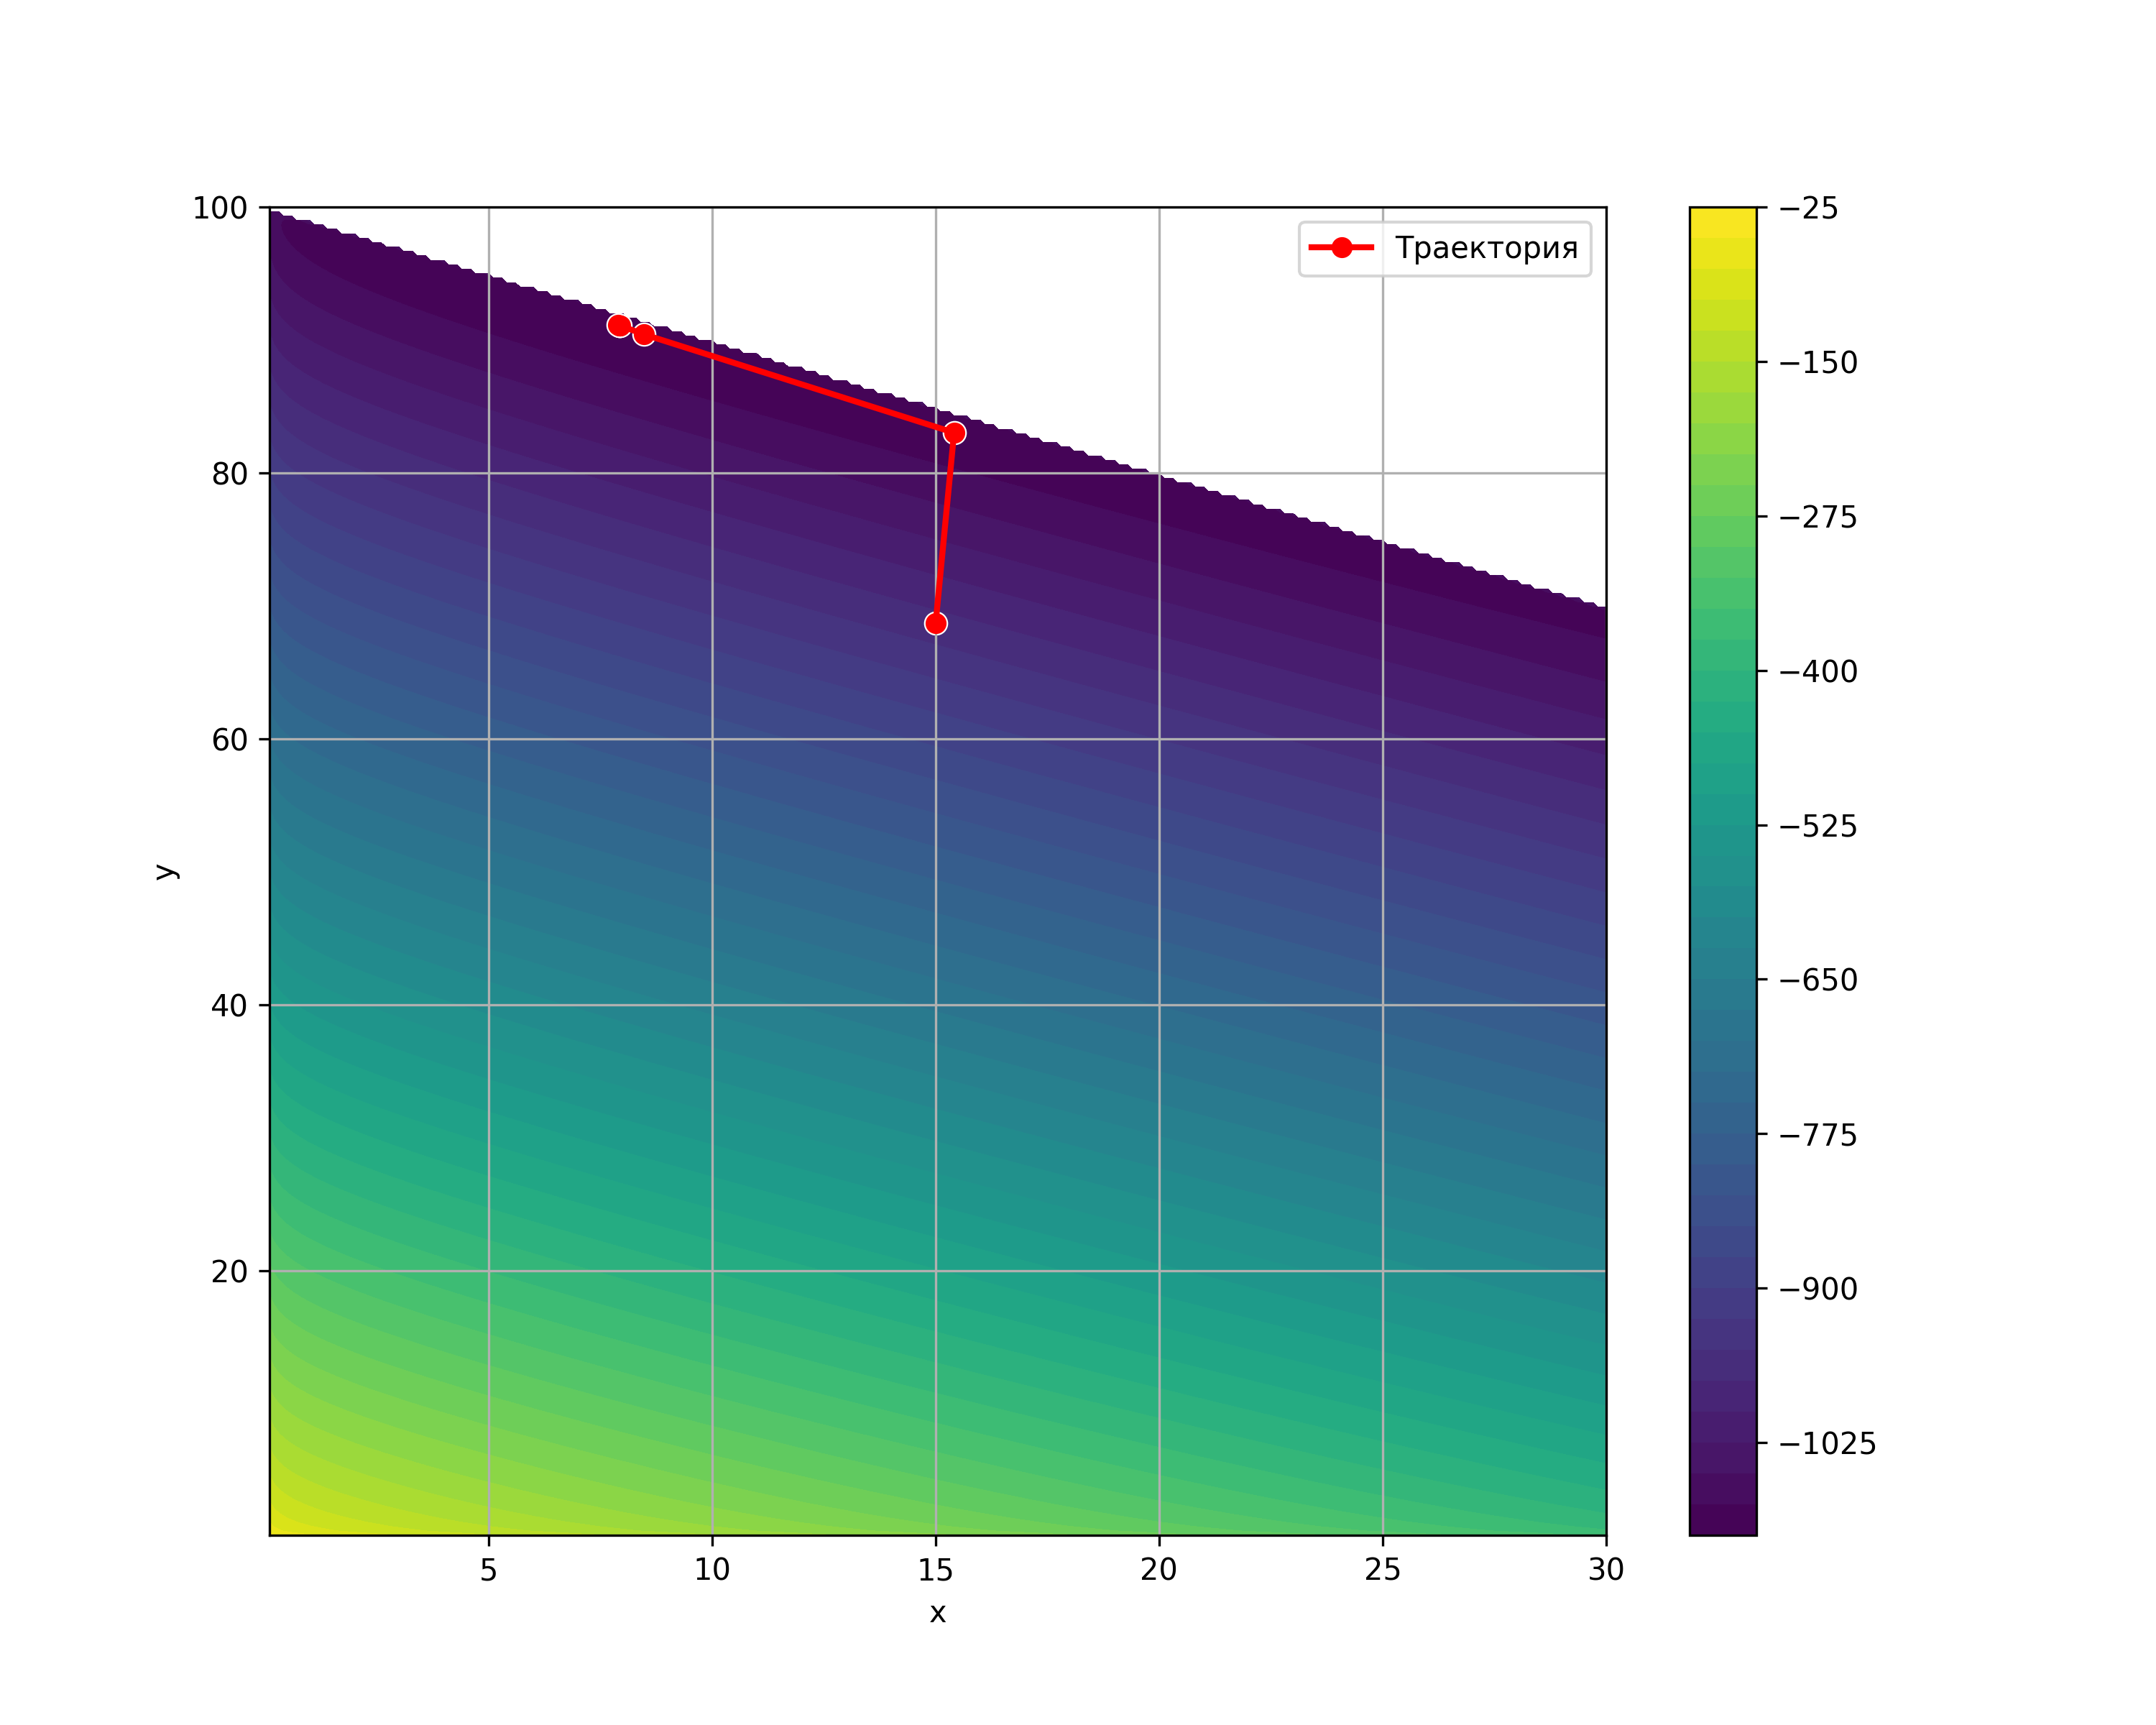
\includegraphics[width=0.49\textwidth]{images/newton_adaptive_trajectory_2.png}
    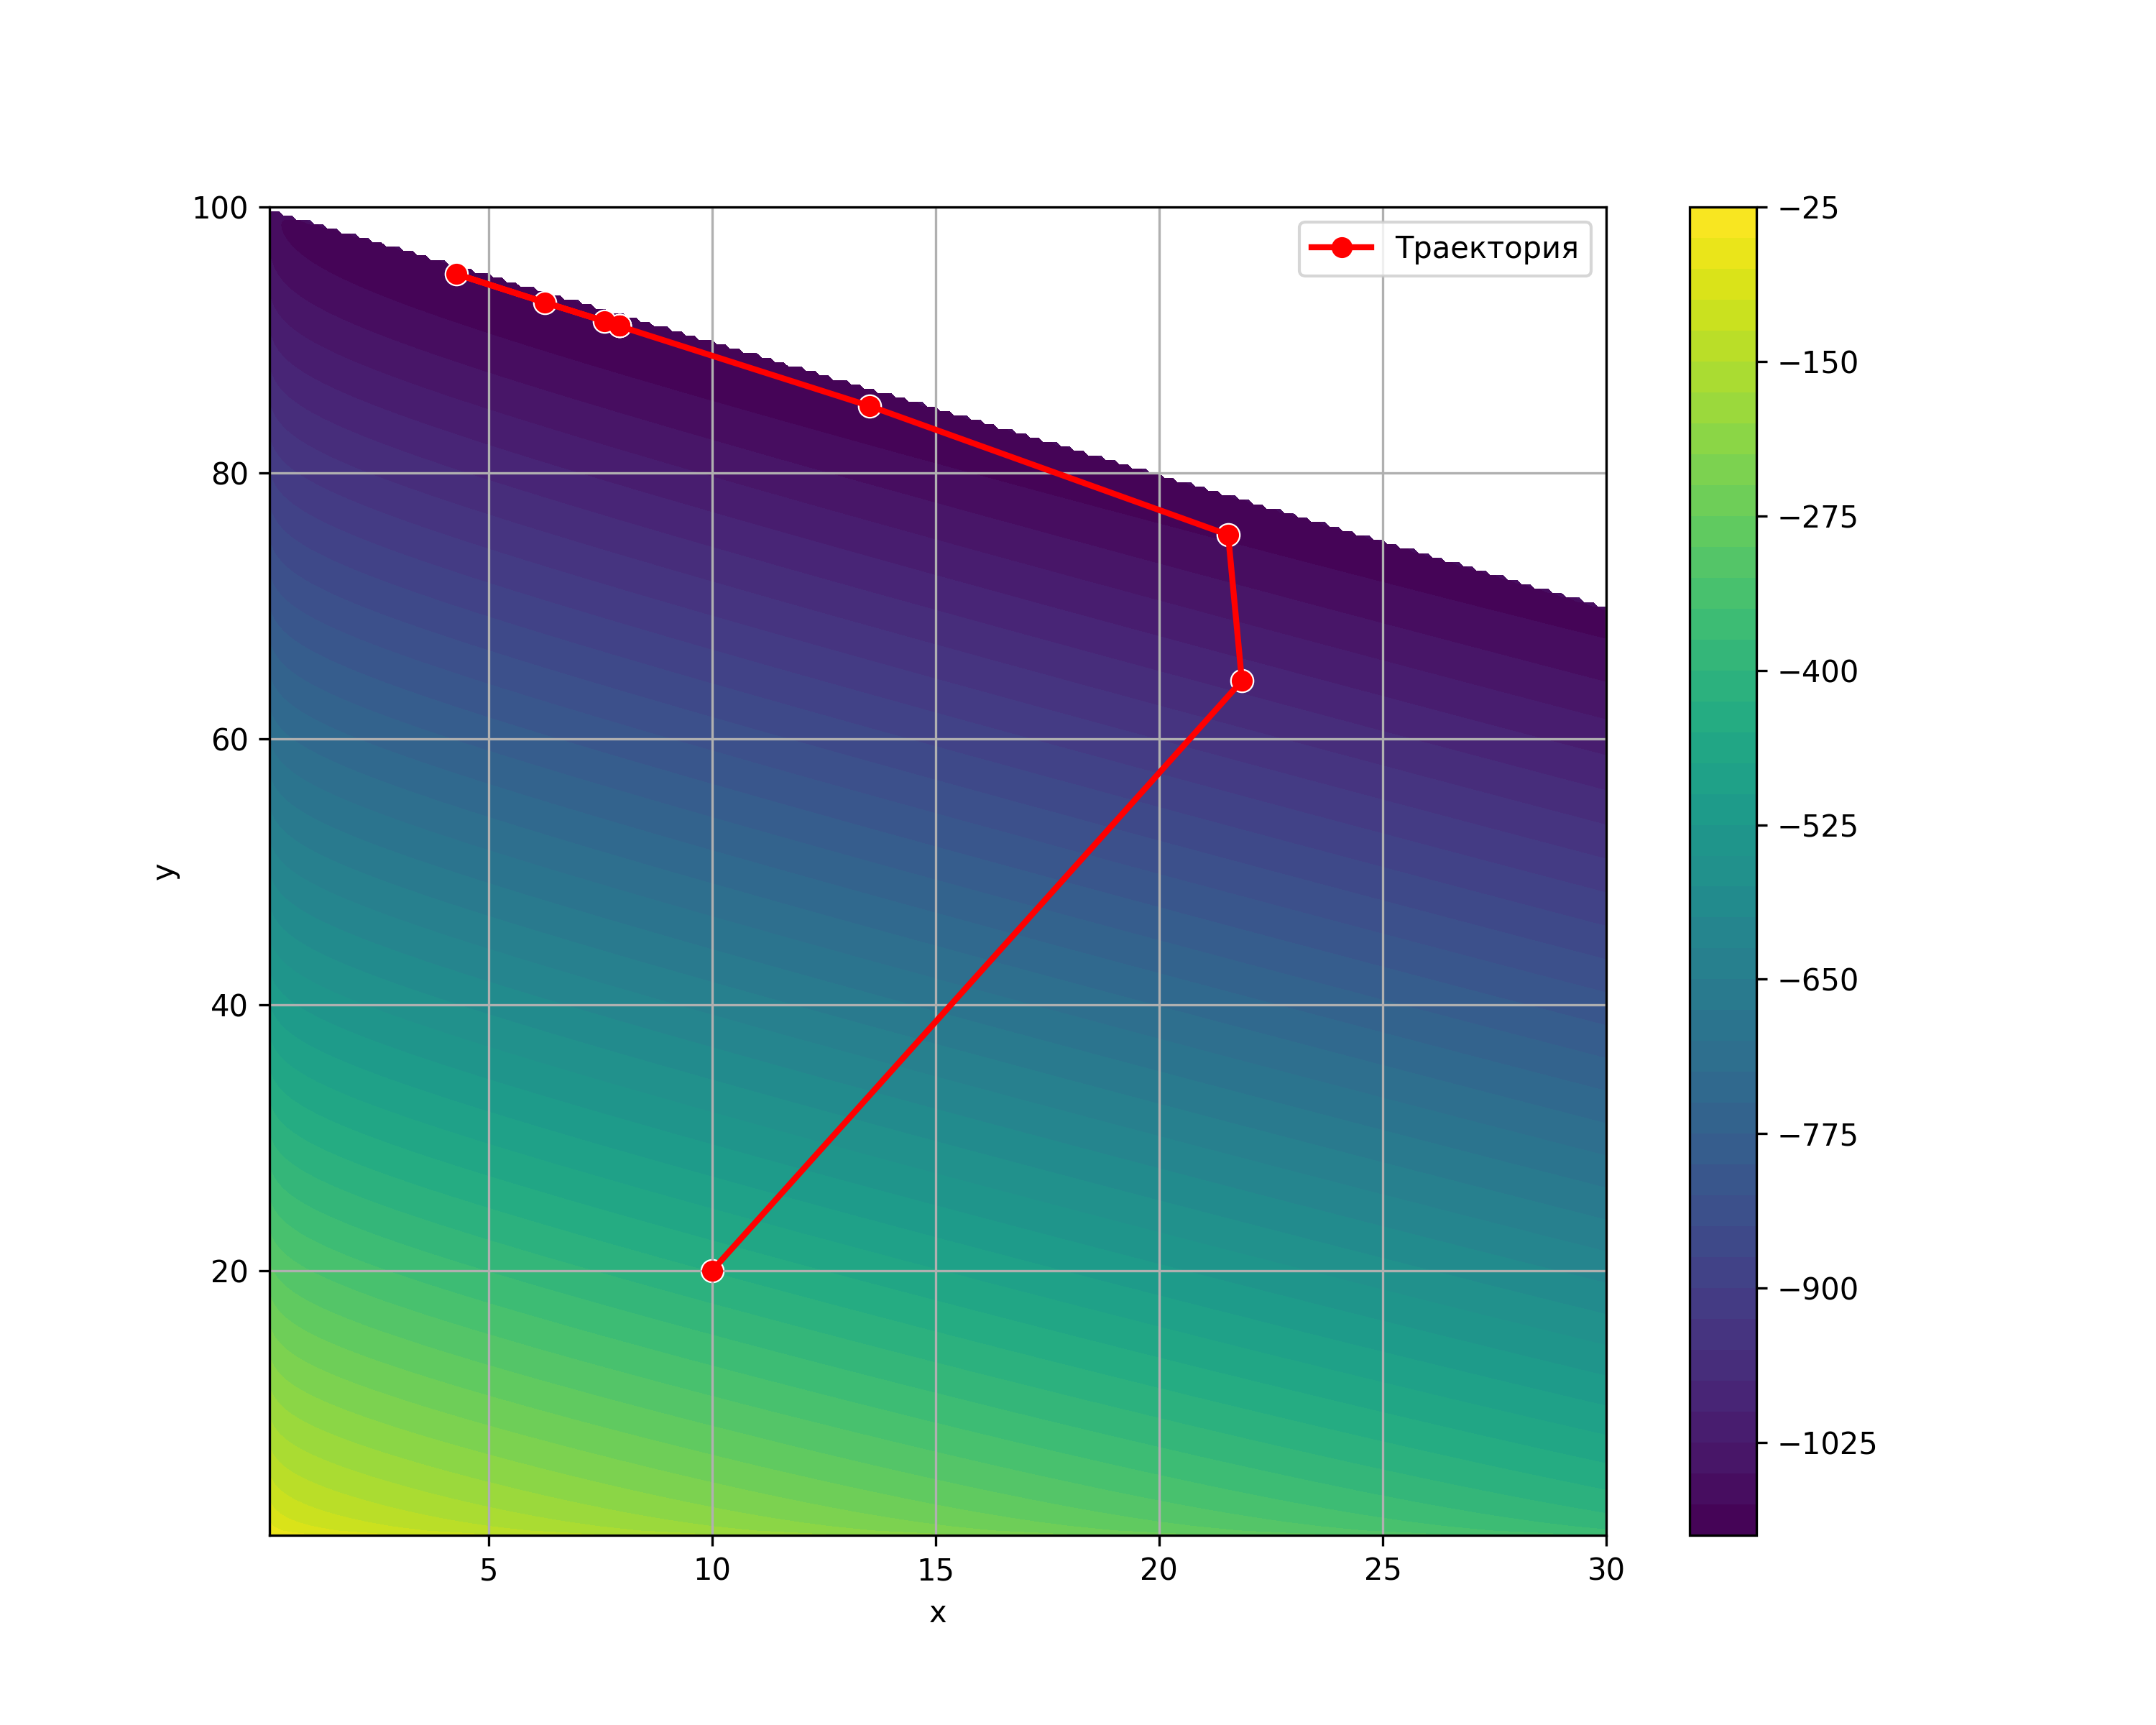
\includegraphics[width=0.49\textwidth]{images/newton_adaptive_trajectory_3.png}
    \caption{Траектории итераций метода Ньютона с адаптивным подбором шага для различных начальных точек.}
  \end{figure}
\noindent Из графиков видно, что при адаптивном подборе шага траектории итераций получаются плавными и аккуратными. Начальные точки независимо от их расположения постепенно сходятся к минимуму, так как шаг подбирается с учетом локальных особенностей функции, что делает метод стабильным даже при старте далеко от оптимума.

\section{Общий вывод}
В ходе работы мы пришли к следующим выводам:
\begin{itemize}
    \item Центральные разностные схемы позволяют достаточно точно вычислять градиент и гессиан, если правильно выбран шаг \(h\).
    \item Для простых функций, например квадратичных, метод Ньютона сходится очень быстро (даже за одну итерацию), что подтверждает его эффективность.
    \item При использовании фиксированного параметра метод может расходиться или «улетать в космос», если начальные точки выбраны неудачно, так как фиксированный параметр не учитывает ограничения функции.
    \item Применение адаптивного подбора параметра значительно улучшает сходимость и делает метод более стабильным.
\end{itemize}

Таким образом, метод Ньютона является мощным инструментом оптимизации, но для успешного его применения необходимо правильно подбирать параметры и учитывать особенности задачи.
\end{document}
